\section{Convergence}

The program requires four arguments:
\begin{enumerate}
    \item The stopping criterion.
    \item The Reynolds number.
    \item The timestep $\Delta t$.
    \item The number of planes in the horizontal and vertical direction $N$.
\end{enumerate}
Each of these four arguments has a major impact on the outcome of the simulation and must therefore be carefully considered. 

The simulation will halt when
\begin{equation}
    \frac{ \text{max} \left( \left| \mathbf{u}^n - \mathbf{u}^{n-1} \right| \right) }{\Delta t} < \text{tol}
\end{equation}
where tol is an abbreviation of tolerance. A tolerance of $1 \cdot 10^{-5}$ turned out to be a reasonable compromise between accuracy and execution time. The Reynolds number was fixed at 1000 to match the benchmark results. The number of planes in the horizontal and vertical direction $N$ was increased from 16 to 64 with three intermediate steps. The timestep $\Delta t$ is highly dependent on $N$; in certain numerical methods, it is crucial to choose the timestep such that the flow does not cover a distance larger than the smallest mesh spacing within $\Delta t$. This condition is known as the Courant–Friedrichs–Lewy (CFL) condition:
\begin{equation}
    C = \frac{u \Delta t}{\Delta x} \leq C_{\text{max}}
\end{equation}
where $C_{\text{max}}$ is typically equal to 1, so
\begin{equation}
    \Delta t \leq \frac{C_{\text{max}} \Delta x}{u}
\end{equation}
While the CFL condition does not nessecarily in this case, it can at least serve as a guideline. The CFL condition turned out to hold within an order of magnitude and the final value of $\Delta t$ was determined by means of trial and error. A timestep that is too large causes the solution to diverge and a timestep that is too small results in unnecessarily slow convergence. The optimal timestep is a value just below the value that would cause the solution to diverge. The parameters used in the creation of the final results are tabulated in Table \ref{tab:results2}.

\begin{table}[h]
    \centering
    \begin{tabular}{rrrrrrr}  
        \toprule
        \# & $N$ & $\Delta t$ & tolerance & Re & iterations & $\text{iterations} \cdot \Delta t$ \\
        \midrule
        1 & 16 & 0.05 & $1 \cdot 10^{-5}$ & 1000 & 1379 & 68.95 \\
        2 & 32 & 0.004 & $1 \cdot 10^{-5}$ & 1000 & 12002 & 48.01 \\
        3 & 48 & 0.0007 & $1 \cdot 10^{-5}$ & 1000 & 56577 & 39.60 \\
        4 & 56 & 0.0004 & $1 \cdot 10^{-5}$ & 1000 & 93111 & 37.24 \\
        5 & 64 & 0.0002 & $1 \cdot 10^{-5}$ & 1000 & ? & ? \\
        \bottomrule
    \end{tabular}
    \caption{Settings for different runs of the simulation.}
    \label{tab:results2} 
\end{table}

It is interesting that the actual simulated time $\text{iterations} \cdot \Delta t$ (see the rightmost column of Table \ref{tab:results2}) converges to around 35 (omitting the word "seconds" here because the time is dimensionless). The more detailed your simulation, the closer the approximation of transport of momentum in the fluid. The simulation converges once the flow field is rotates steadily, which requires transport of momentum from the boundaries to the center of the domain.

\section{Stream Function}

The stream function $\tilde{\psi}$ is defined such that the difference $\Delta \tilde{\psi}$ between two streamlines is equal to the mass flux between two streamlines. This fact allows us to compute the stream function based on the values of flux along the line segments. The outer-oriented line segments $\tilde{u}_{i,j}$ and $\tilde{v}_{i,j}$ represent flux in the form:
\begin{flalign}
    \stepcounter{equation}
    \tag{{\theequation}a}
    \label{eq:results1}
    & & \tilde{u}_{i,j} = \int_{y_{i,j}}^{y_{i,j+1}} \mathbf{u} \cdot  \mathbf{\hat{n}} \, dy && \\
    \tag{{\theequation}b}
    \label{eq:results2}
    &\text{and}& \tilde{v}_{i,j} = \int_{x_{i,j}}^{x_{i+1,j}} \mathbf{u} \cdot \mathbf{\hat{n}} \, dx &&
\end{flalign}
where $\mathbf{\hat{n}}$ denotes the normal vector along the line segment. Thus, computing the stream function is a simply matter of assuming that the stream function has a value of zero at the boundaries and using either Equation \eqref{eq:results1} or Equation \eqref{eq:results2} to compute the unknowns in the remainder of the domain.

Figure \ref{fig:SFN64} shows an interpolated contour plot of the stream function for $N = 64$, $\text{Re} = 1000$, $\Delta t = 0.0002$, and $\text{tol} = 1 \cdot 10^{-5}$. Figure \ref{fig:benchmarkSFN64} shows the benchmark result from \parencite{botella1998benchmark}. The contour levels associated with the labels $a$--$j$ in Figure \ref{fig:benchmarkSFN64} can be found in Table 7 of \parencite{botella1998benchmark}. The two figures are, for all intents and purposes, identical. Figure \ref{fig:allsf} shows plots of the stream function for $N = 16$, $N = 32$, $N = 48$, $N = 56$, and $N = 64$ without interpolation as well as the benchmark result.

\section{Vorticity}

Plotting the vorticity requires no post-processing. Figure \ref{fig:VN64} shows a contour plot of the stream function for $N = 64$, $\text{Re} = 1000$, $\Delta t = 0.0002$, and $\text{tol} = 1 \cdot 10^{-5}$. Figure \ref{fig:benchmarkVN64} shows the benchmark result from \parencite{botella1998benchmark}. The contour levels associated with the labels $a$--$k$ in Figure \ref{fig:benchmarkVN64} can be found in Table 8 of \parencite{botella1998benchmark}.

The swirl in the center of the velocity plot (line $d$ in the benchmark result) appears to be different from the benchmark. Aside of the center swirl, the two images are practically identical. The difference is most likely caused by differences in mesh density and tolerance. For example, the benchmarks were created with $N = 128$ and the tolerance may have been set to a smaller number than during the creation of these results. Figure \ref{fig:allvorticity} shows vorticity plots for $N = 16$, $N = 32$, $N = 48$, $N = 56$, and $N = 64$ without interpolation as well as the benchmark result. These plots support the argument that the difference in mesh density $N$ is likely the reason for the difference with the benchmark results; the center swirl is affected most when adjusting $N$.

\section{Pressure}

Computing the pressure does require some additional processing. We are interested in the static pressure $p$ rather than the total pressure $P$. Thus, 
\begin{equation}
    p = P - \frac{1}{2} \left\Vert \mathbf{u} \right\Vert^2
\end{equation}
The velocities at the line segments can be found by dividing the circulation by the length of the respective line segments and taking the average of the velocities around $P_{i,j}$. We therefore have
\begin{equation}
    \left\Vert \mathbf{u} \right\Vert_{i,j} = \sqrt{\left[ \frac{1}{2} \left( \frac{u_{i-1,j}}{h_{i-1}} + \frac{u_{i,j}}{h_i} \right) \right]^2 + \left[ \frac{1}{2} \left( \frac{v_{i,j-1}}{h_{j-1}} + \frac{v_{i,j}}{h_j} \right) \right]^2}
\end{equation}
and the static pressure $p$ can be determined up to a constant. The pressure can only be determined up to a constant because the flow is governed by differences in \emph{static} pressure; the total pressure is irrelevant. To reproduce the plot in \parencite{botella1998benchmark}, the static pressure must be scaled such that it equals zero at the center of the domain.

Figure \ref{fig:PN64} shows a contour plot of the stream function for $N = 64$, $\text{Re} = 1000$, $\Delta t = 0.0002$, and $\text{tol} = 1 \cdot 10^{-5}$. Figure \ref{fig:benchmarkPN64} shows the benchmark result from \parencite{botella1998benchmark}. The contour levels associated with the labels $a$--$j$ in Figure \ref{fig:benchmarkPN64} can be found in Table 8 of \parencite{botella1998benchmark}. The static pressure plot shows the same overal pattern as the benchmark results, but the lines are slightly displaced. The difference is causes by the fact that the mesh densities are different ($N = 128$ versus $N = 64$) and the constant that is subtracted from the static pressure may have been different. Figure \ref{fig:allpressure} shows plots of the stream function for $N = 16$, $N = 32$, $N = 48$, $N = 56$, and $N = 64$ without interpolation as well as the benchmark result. The match with the benchmark results is rather poor for low values of $N$.

\section{Code Optimizations}

The results of the optimizations suggested in Chapter \ref{cha:code} are tabulated in Table \ref{tab:results1}. The baseline version of the program is the skeleton code supplied with this assignment. The largest single cumulative factor of speedup with respect to the baseline version is 343.89. To put that into perspective, a speedup of 343.89 makes a simulation that takes one week to run finish in just under half an hour.

The largest single relative factor of speedup is 23.42. This is quite a remarkable factor of speedup given that it is merely the result of simply rearranging parts of the code. This proves yet again that the principle of "do less work" along with using common sense goes a long way in optimizing slow pieces of code.

\begin{table}[h]
    \centering
    \begin{tabular}{llrrr}  
        \toprule
        \# & Version & Execution time & Speedup (rel.) & Speedup (cum.) \\
        \midrule
        1 & Baseline & 3 h 37 m 48 s & 1.00 & 1.00 \\
        2 & Rearranged code & 9 m 18 s & 23.42 & 23.42 \\
        3 & No factorization stage & 3 m 11 s & 2.92 & 68.42 \\
        4 & Sparse matrix storage & 1 m 55 s & 1.66 & 113.63 \\
        5 & Double-precision in \texttt{C} & 1 m 7 s & 1.72 & 195.04 \\
        6 & Single-precision in \texttt{C} & 38 s & 1.76 & 343.89 \\
        \bottomrule
    \end{tabular}
    \caption{Execution time and factors of speedup for $N = 32$, $\text{Re} = 1000$, $\Delta t = 0.004$, and $\text{tol} = 1 \cdot 10^{-5}$ on an Intel Core i5-2400 with four CPU cores clocked at 3100 MHz (CPU throttling and turbo disabled).}
    \label{tab:results1} 
\end{table}

\section{Integrated Vorticity}

The integrated vorticity is more or less constant, regardless of the value of $N$ used to run the simulation. The integrated viscosity grows quadratically as a function of the Reynolds number. Here is why: for a general fluid, vorticity is twice the mean angular velocity and is therefore related to angular momentum. Angular momentum can neither be created nor destroyed and must be constant in a \emph{closed} system. However, the lid-driven cavity is \emph{not} a closed system because energy is continuously added to the system by the moving boundary. At $t = 0$, the integrated angular momentum of the system is zero. The moving boundary adds energy (and therefore angular momentum) to the system until the viscous dissipation is able to dissipate the energy that is added to the system by the boundary. This is when an equilibrium settles in and the system rotates steadily (aside of unsteady fluctuations). A high Reynolds number implies that the fluid is viscous and that viscous dissipation occurs at small length scales. As a result, a high Reynolds number allows the system to build up more angular momentum before the viscous dissipation can provide a sink for the energy that is added to the system. 

\section{Turbulence}

One question I have been asking myself ever since starting this assignment is: why does the simulation converge? After all, we are simulating the unsteady viscous Navier-Stokes equations and not some time-averaged equations. The simulation converges because the Reynolds number is very low and the flow is entirely laminar. A low Reynolds number implies that the fluid is relatively "sluggish", that the viscous dissipation takes place at relatively large scales, and that small unsteady vortices are suppressed. Trial runs with a far larger Reynolds number show that the rate of convergence drops dramatically (that is, the solution does not converge) and starts fluctuating wildly. The wild fluctuation can be attributed to the large and small vortices that are continuously being created and destroyed.

\begin{figure}[p]
    \centering
    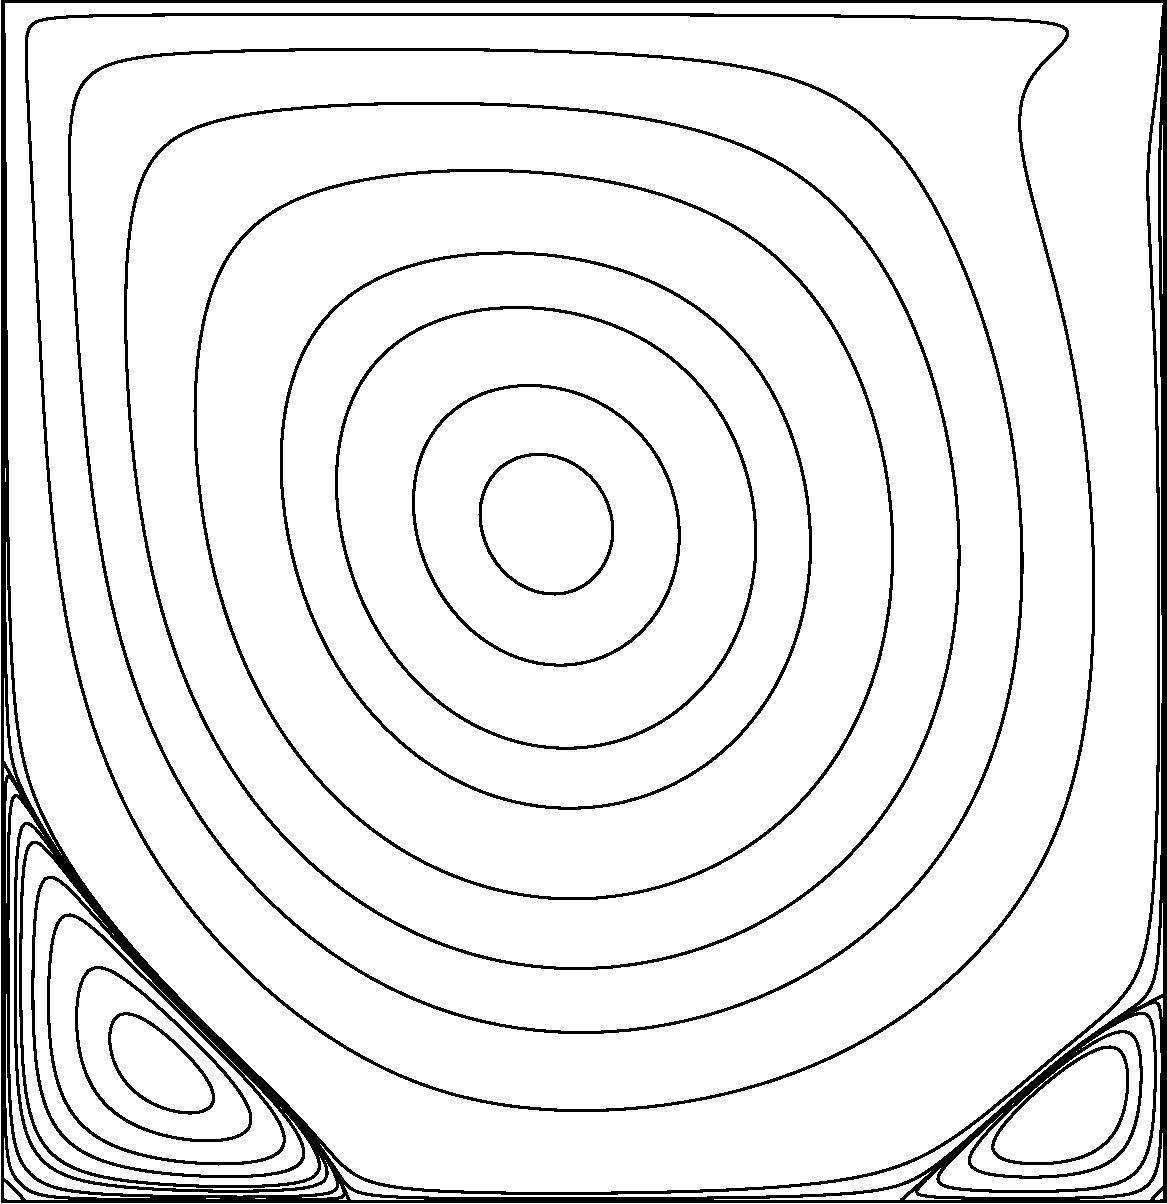
\includegraphics[width=0.85\textwidth]{Images/streamFunction.pdf}
    \caption{Stream function for $N = 64$, $\text{Re} = 1000$, $\Delta t = 0.0002$, and $\text{tol} = 1 \cdot 10^{-5}$.}
    \label{fig:SFN64}
\end{figure}

\begin{figure}[p]
    \centering
    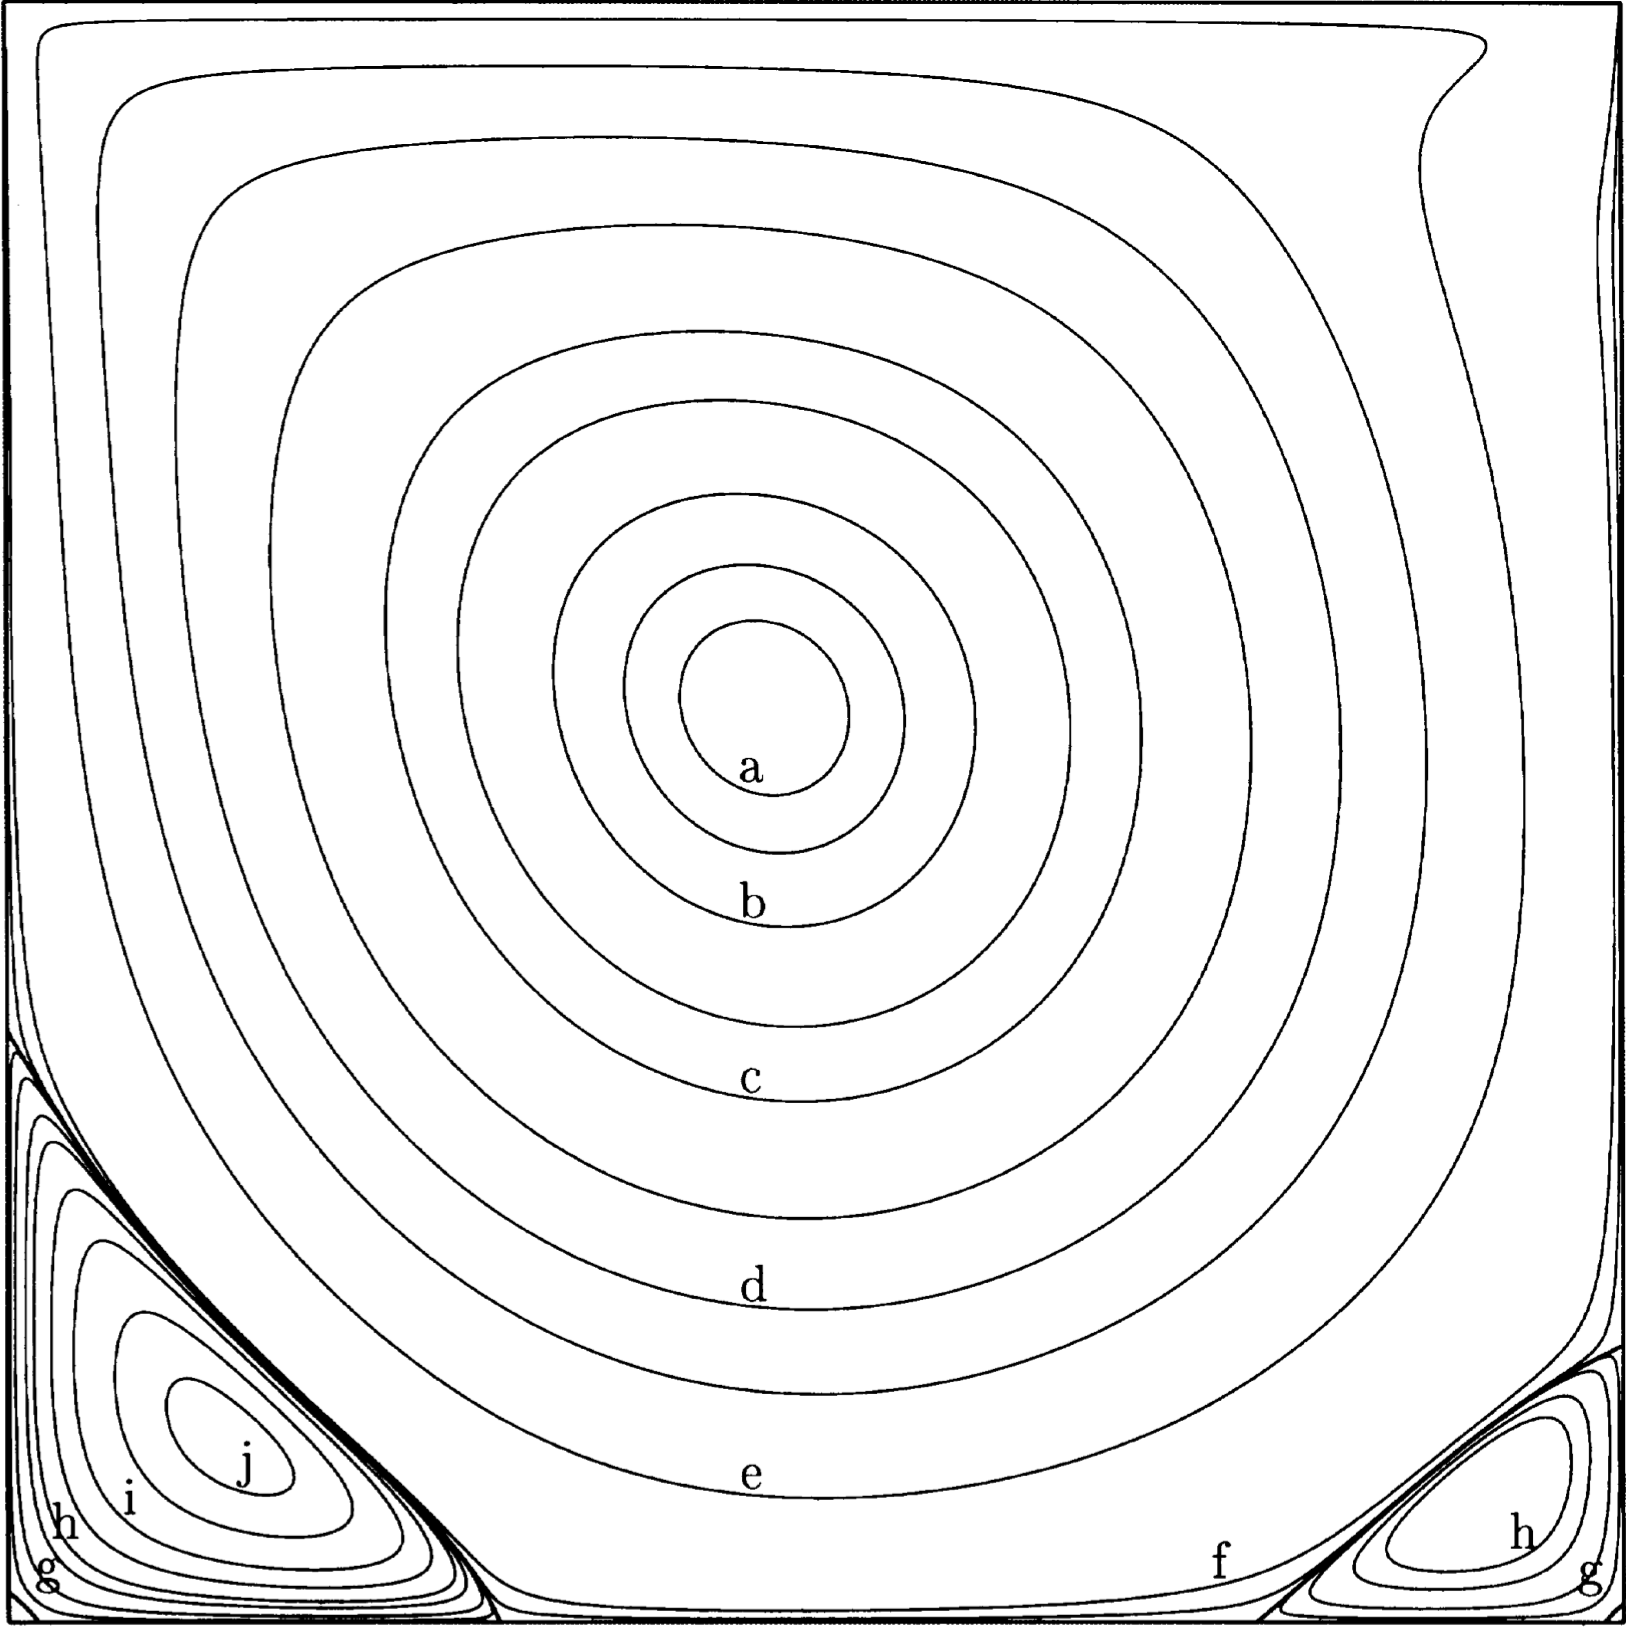
\includegraphics[width=0.85\textwidth]{Images/streamFunction.png}
    \caption{Benchmark stream function for $\text{Re} = 1000$ \parencite{botella1998benchmark}.}
    \label{fig:benchmarkSFN64}
\end{figure}

\begin{figure}[p]
    \centering
    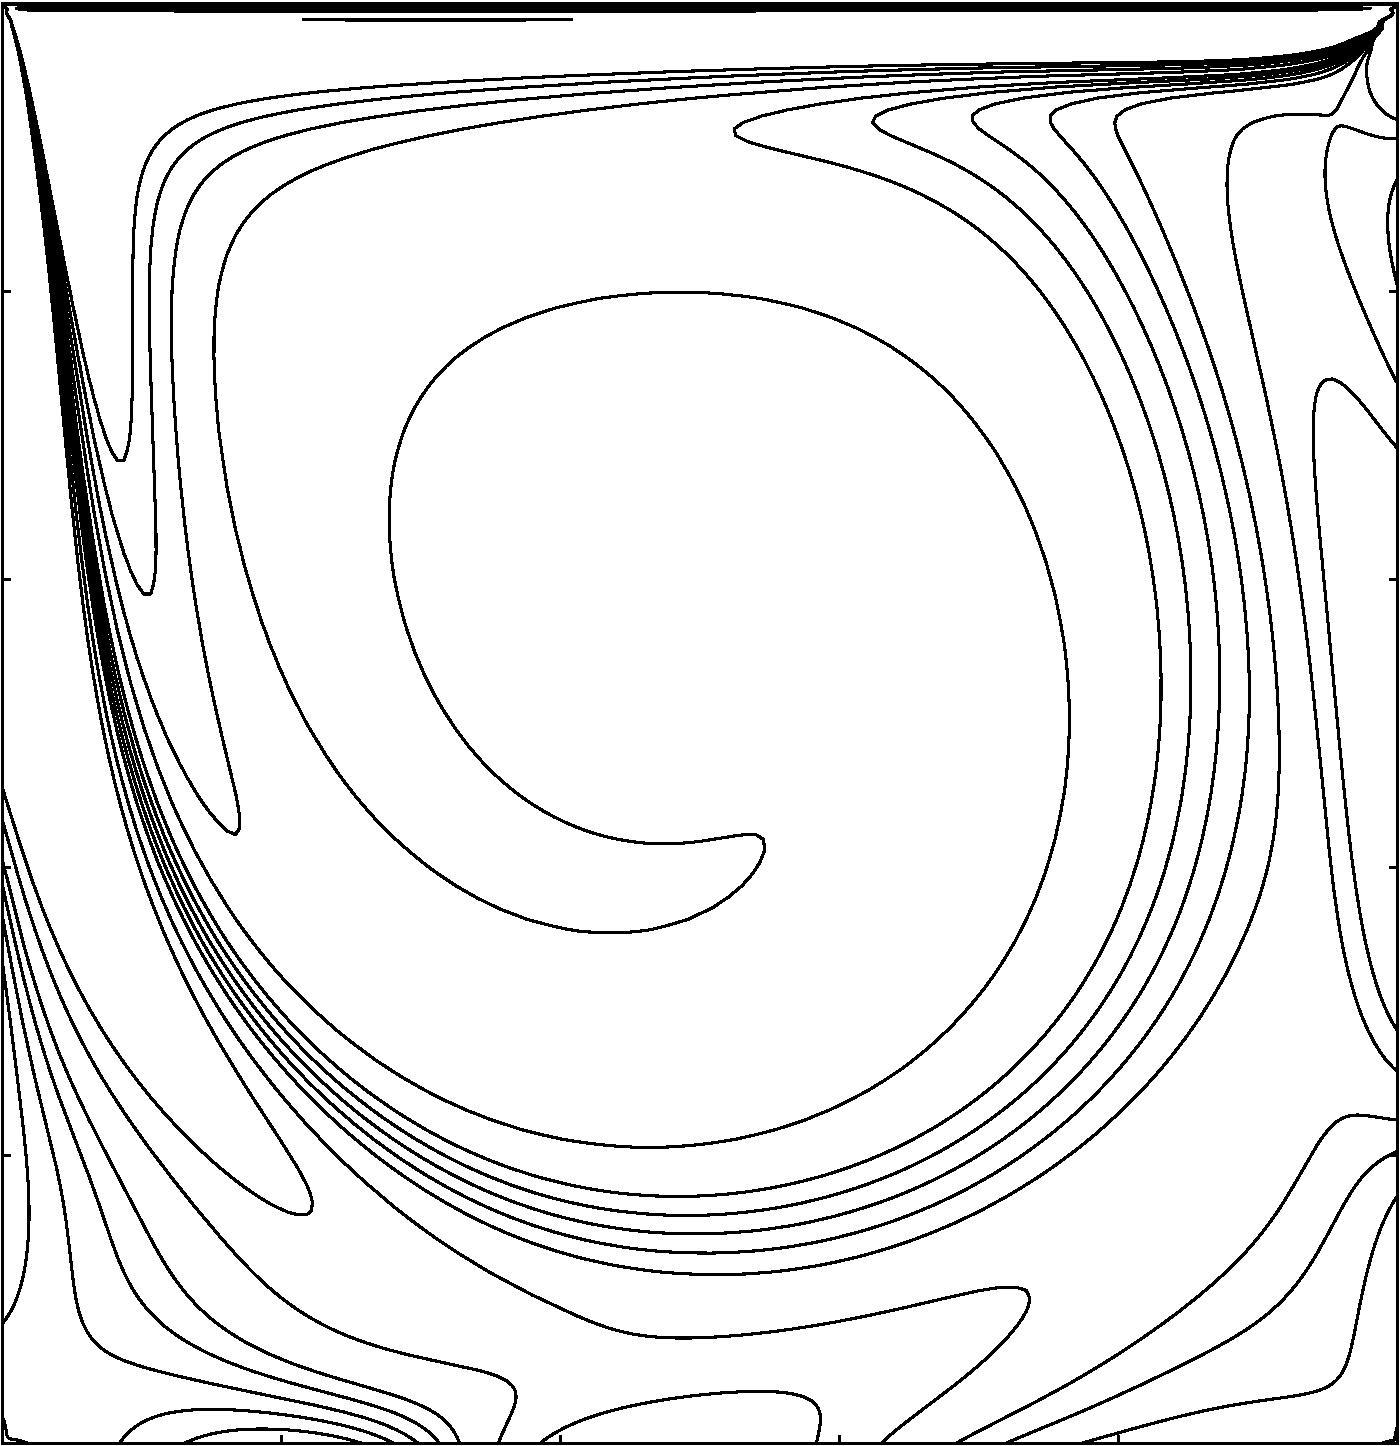
\includegraphics[width=0.85\textwidth]{Images/vorticity.pdf}
    \caption{Vorticity for $N = 64$, $\text{Re} = 1000$, $\Delta t = 0.0002$, and $\text{tol} = 1 \cdot 10^{-5}$.}
    \label{fig:VN64}
\end{figure}

\begin{figure}[p]
    \centering
    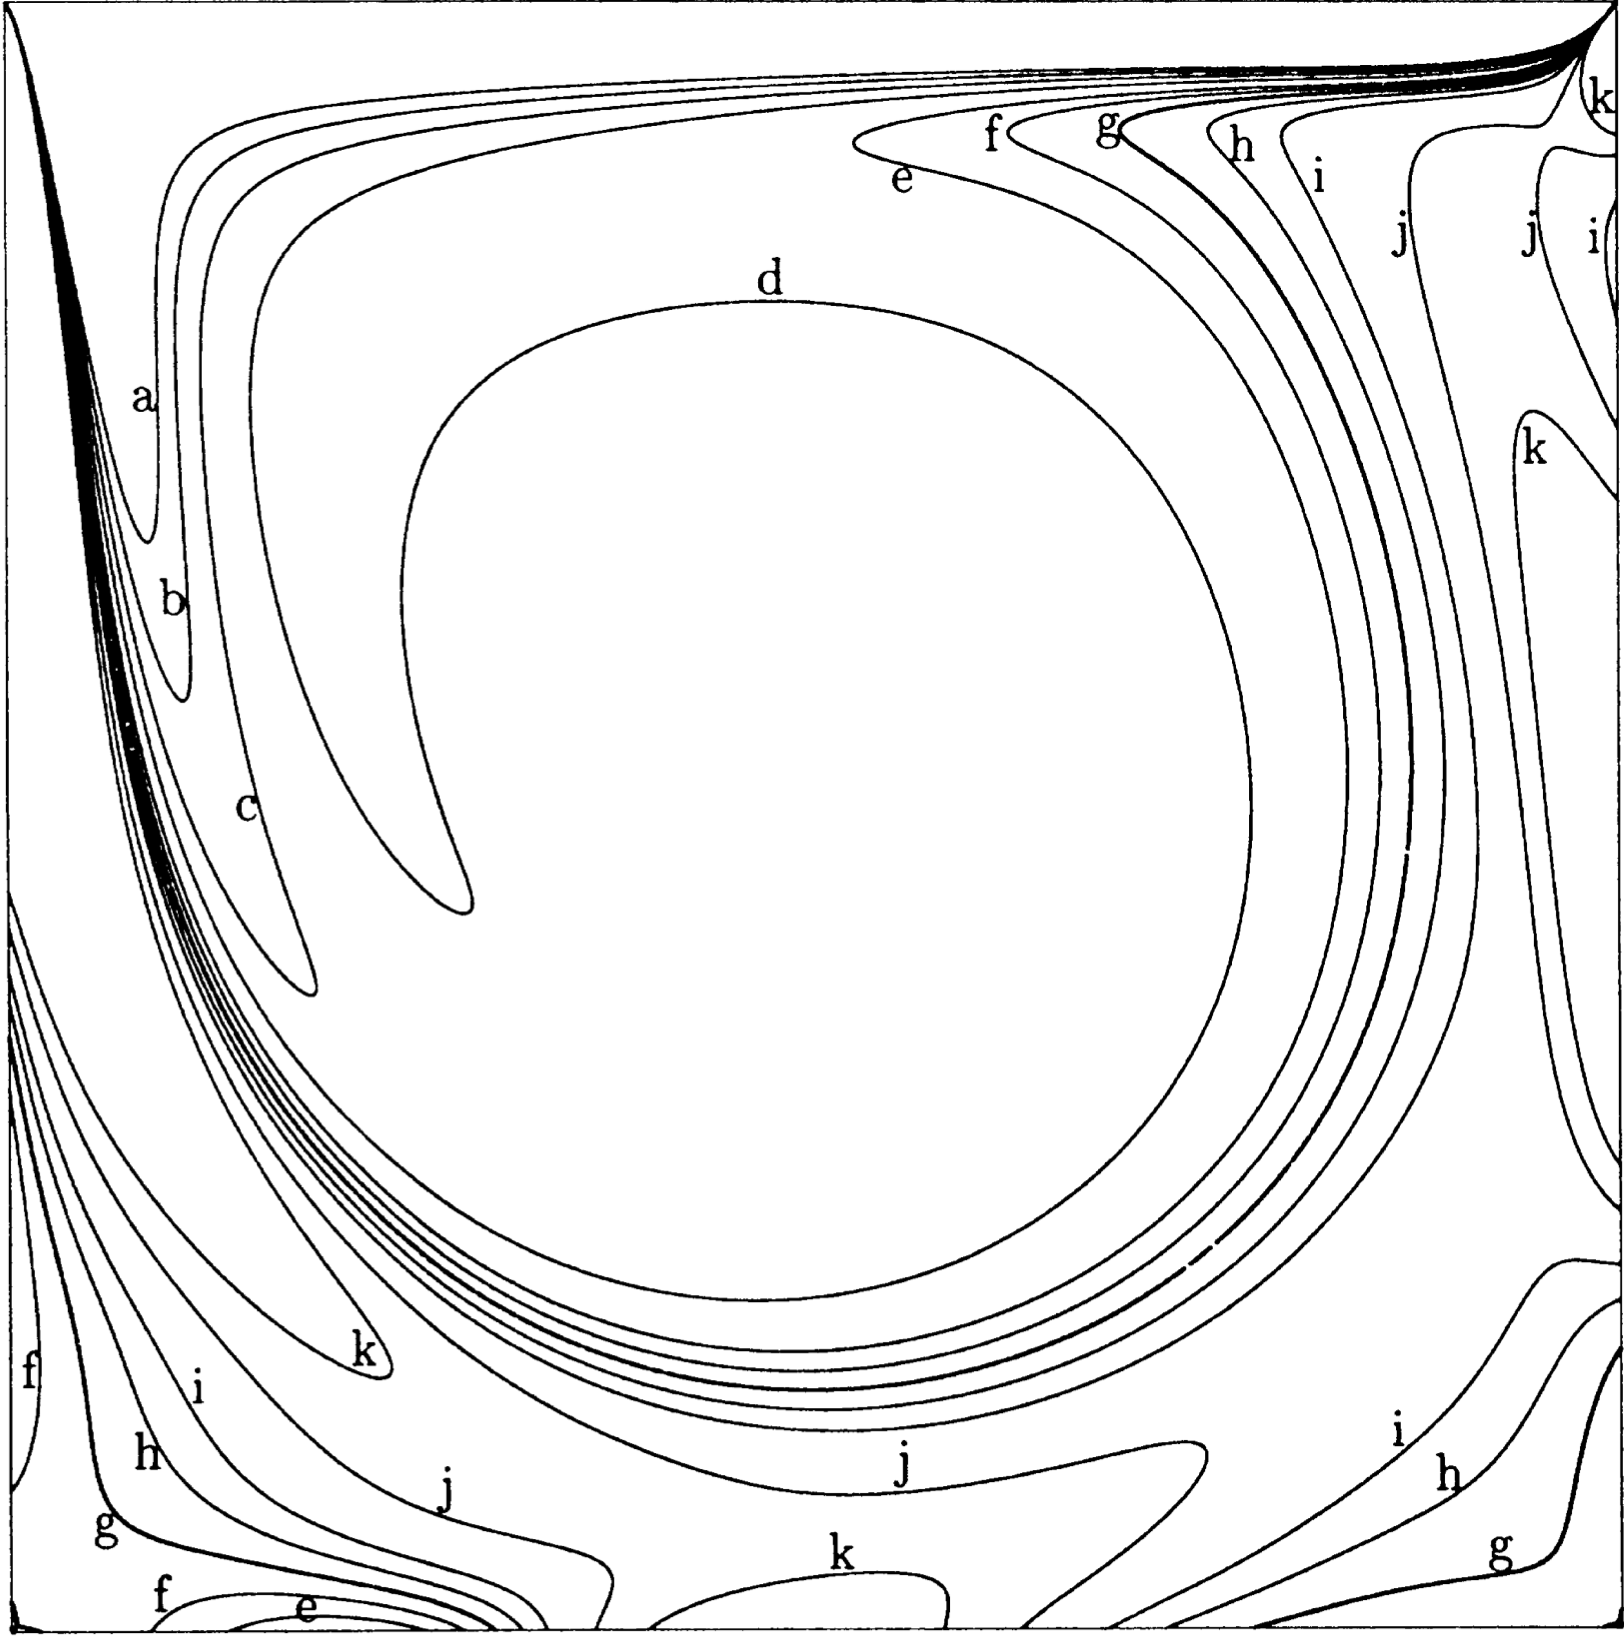
\includegraphics[width=0.85\textwidth]{Images/vorticity.png}
    \caption{Benchmark vorticity for $\text{Re} = 1000$ \parencite{botella1998benchmark}.}
    \label{fig:benchmarkVN64}
\end{figure}

\begin{figure}[p]
    \centering
    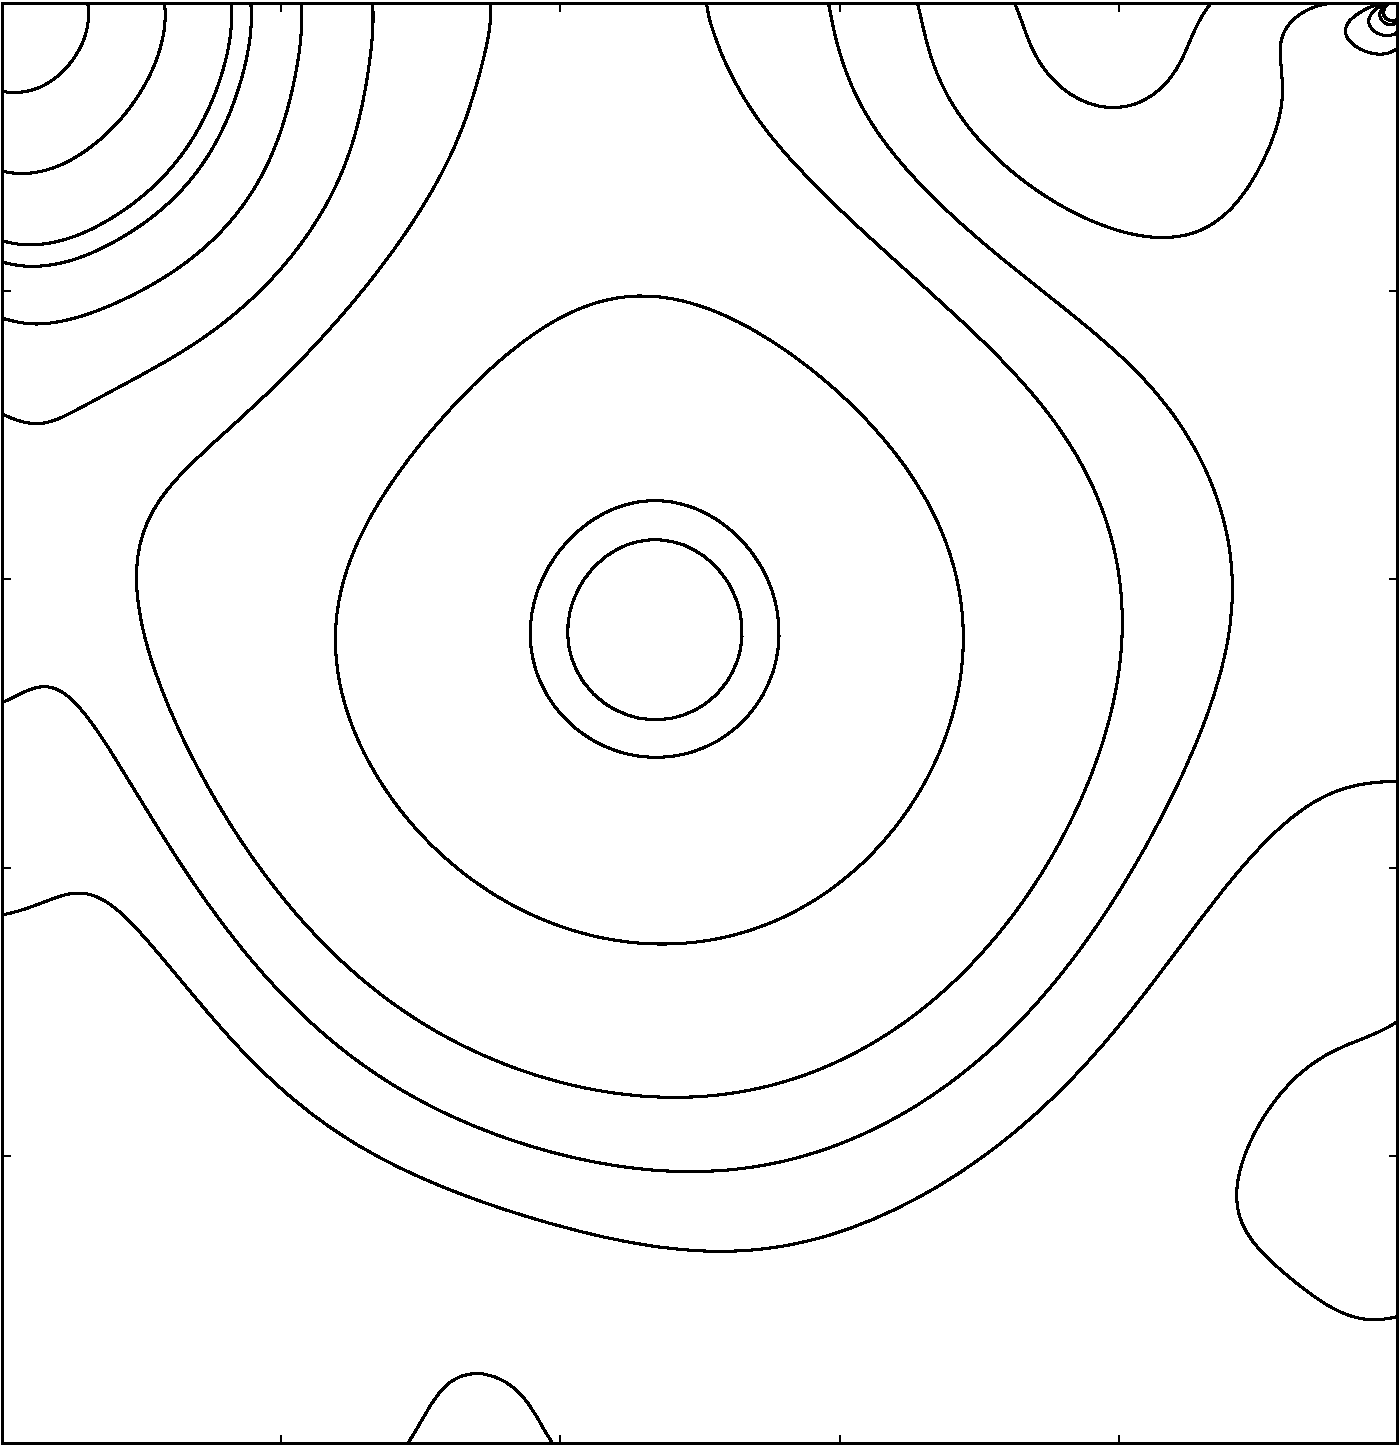
\includegraphics[width=0.85\textwidth]{Images/pressure.pdf}
    \caption{Pressure for $N = 64$, $\text{Re} = 1000$, $\Delta t = 0.0002$, and $\text{tol} = 1 \cdot 10^{-5}$.}
    \label{fig:PN64}
\end{figure}

\begin{figure}[p]
    \centering
    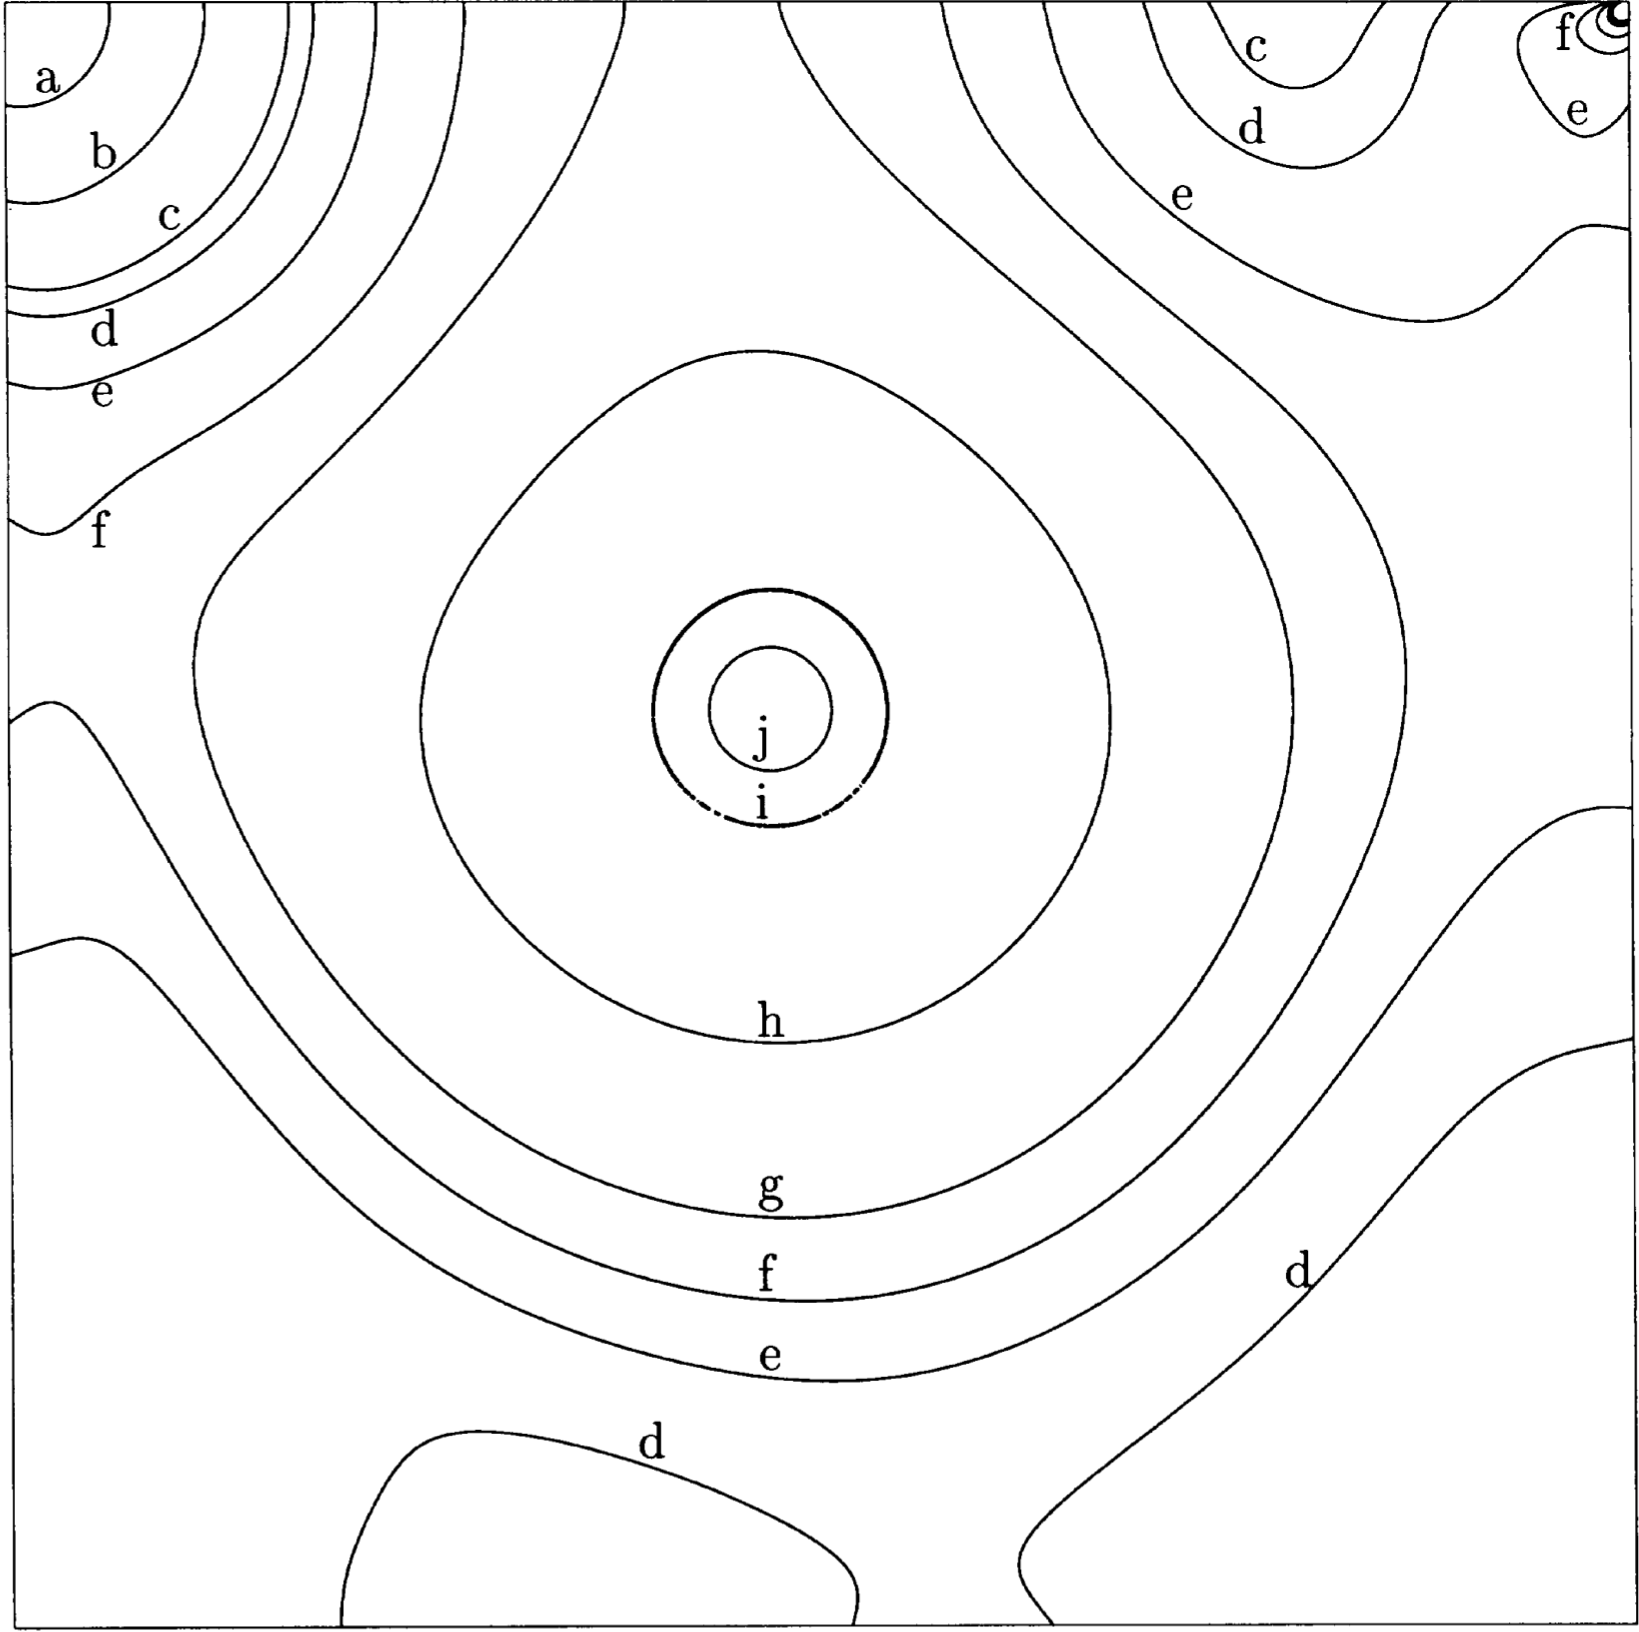
\includegraphics[width=0.85\textwidth]{Images/pressure.png}
    \caption{Benchmark pressure for $\text{Re} = 1000$ \parencite{botella1998benchmark}.}
    \label{fig:benchmarkPN64}
\end{figure}

\begin{figure}[p]
    \centering
    \begin{subfigure}[b]{0.49\textwidth}
        \centering{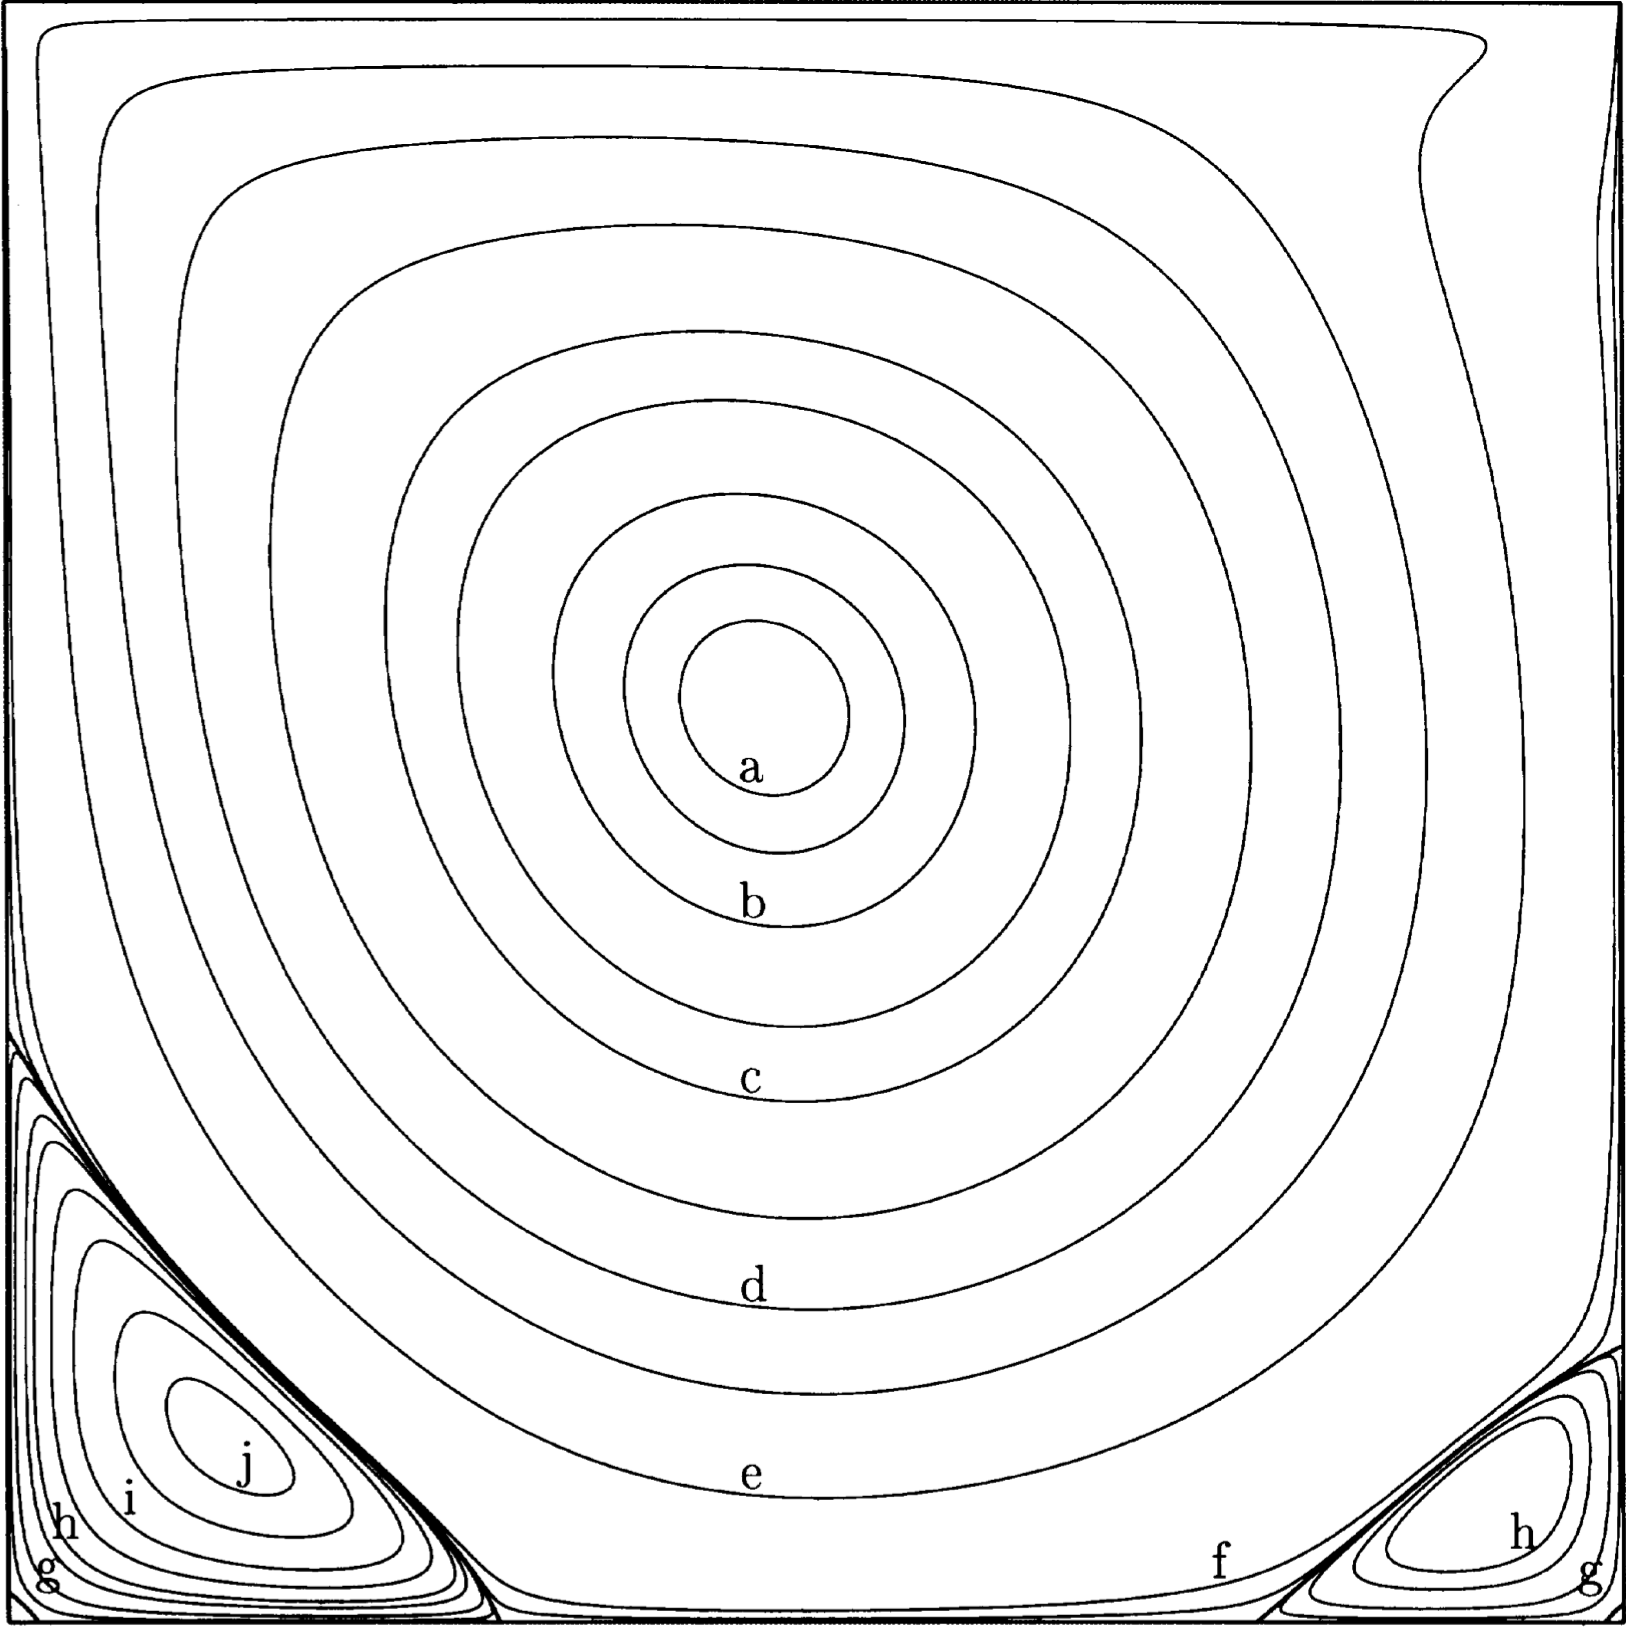
\includegraphics[width=0.95\linewidth]{Images/streamFunction.png}}
	    \caption{Benchmark}
    	\label{fig:sfa}
    \end{subfigure}
    % This comment avoids line break...
    \begin{subfigure}[b]{0.49\textwidth}
        \centering{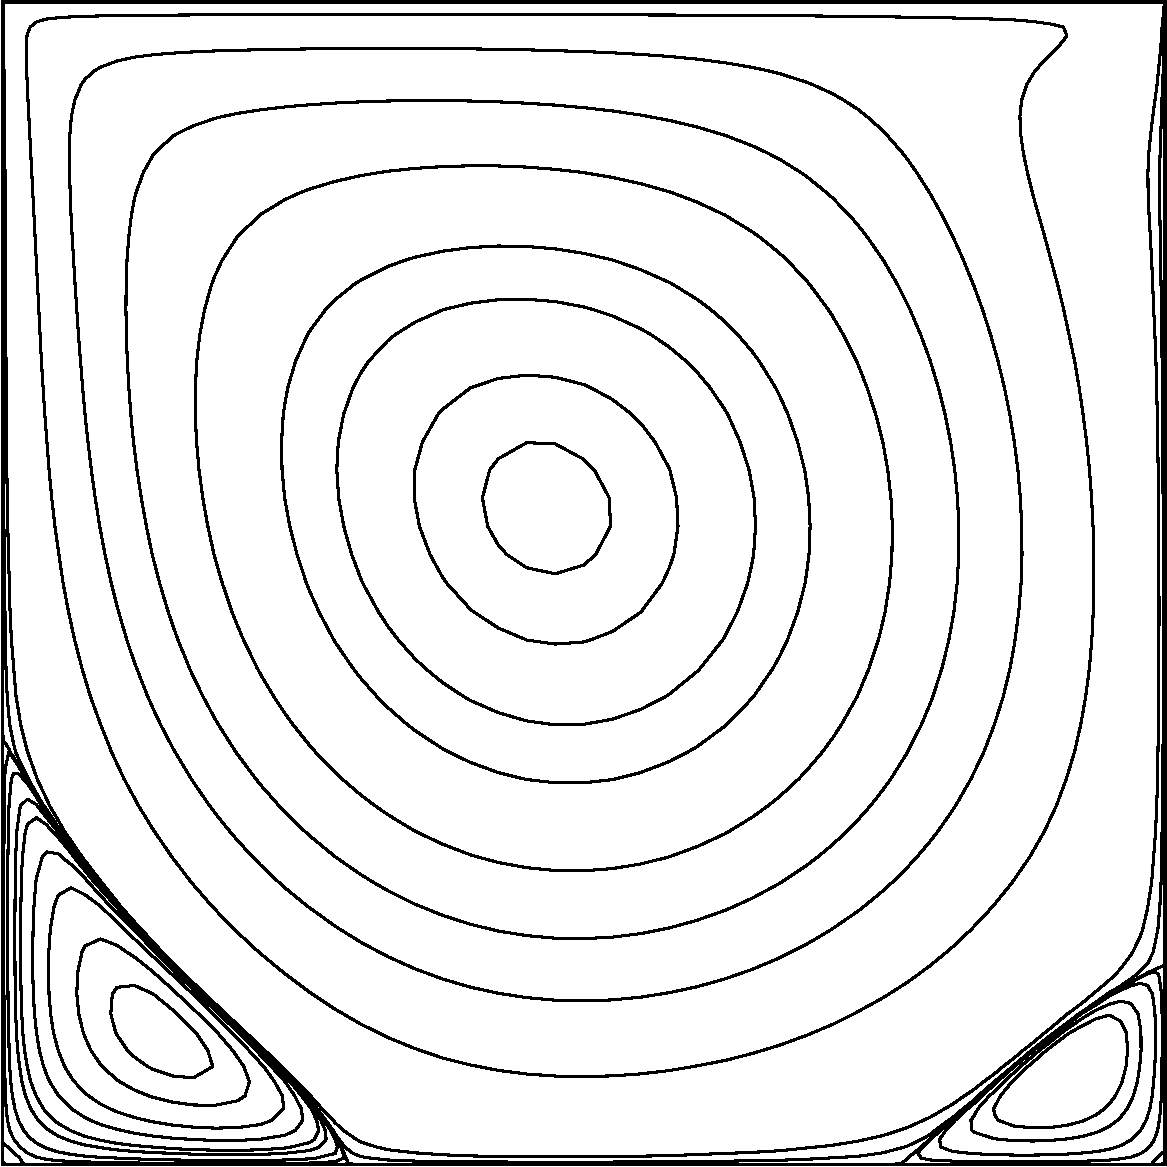
\includegraphics[width=0.95\linewidth]{Images/streamFunction64.pdf}}
	    \caption{$N = 64$}
    	\label{fig:sfb}
    \end{subfigure}
    
    \vspace{1cm}
    
    \begin{subfigure}[b]{0.49\textwidth}
        \centering{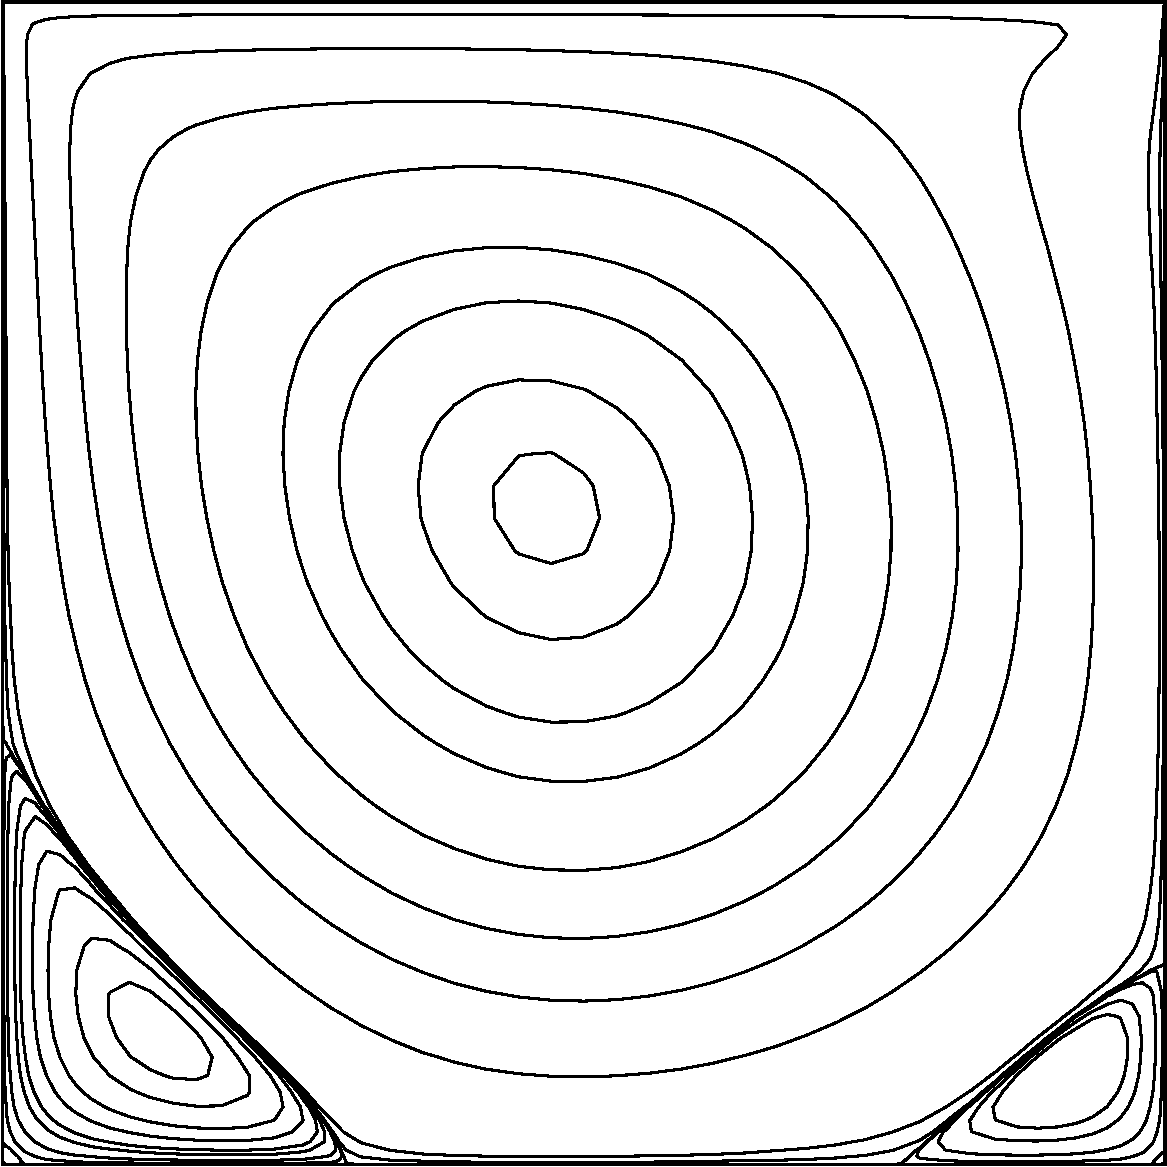
\includegraphics[width=0.95\linewidth]{Images/streamFunction56.pdf}}
	    \caption{$N = 56$}
    	\label{fig:sfc}
    \end{subfigure}
    % This comment avoids line break...
    \begin{subfigure}[b]{0.49\textwidth}
        \centering{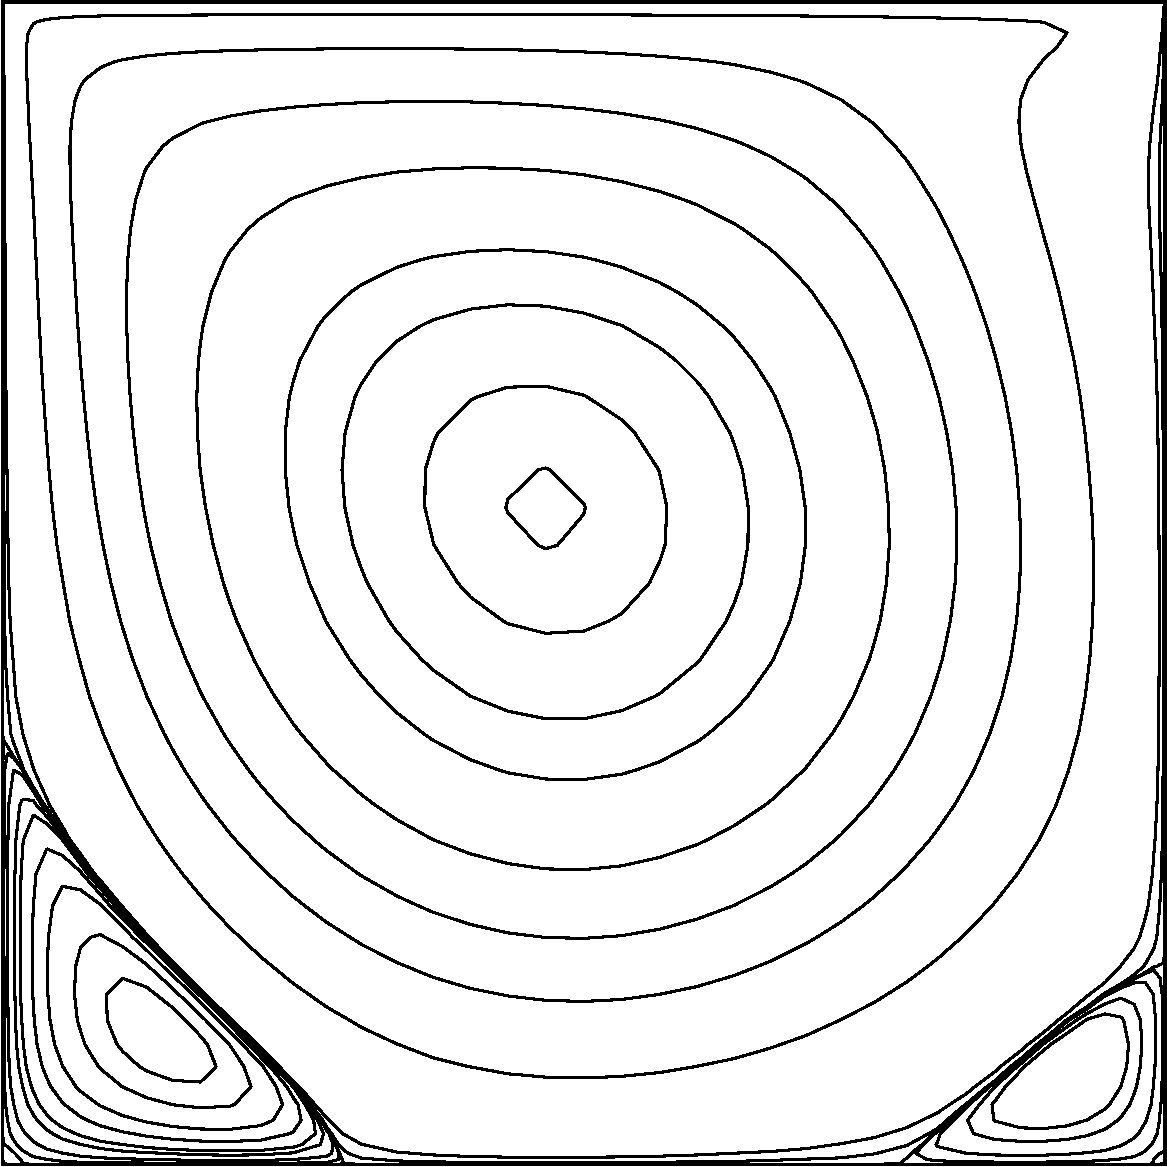
\includegraphics[width=0.95\linewidth]{Images/streamFunction48.pdf}}
	    \caption{$N = 48$}
    	\label{fig:sfd}
    \end{subfigure}
    
    \vspace{1cm}
    
    \begin{subfigure}[b]{0.49\textwidth}
        \centering{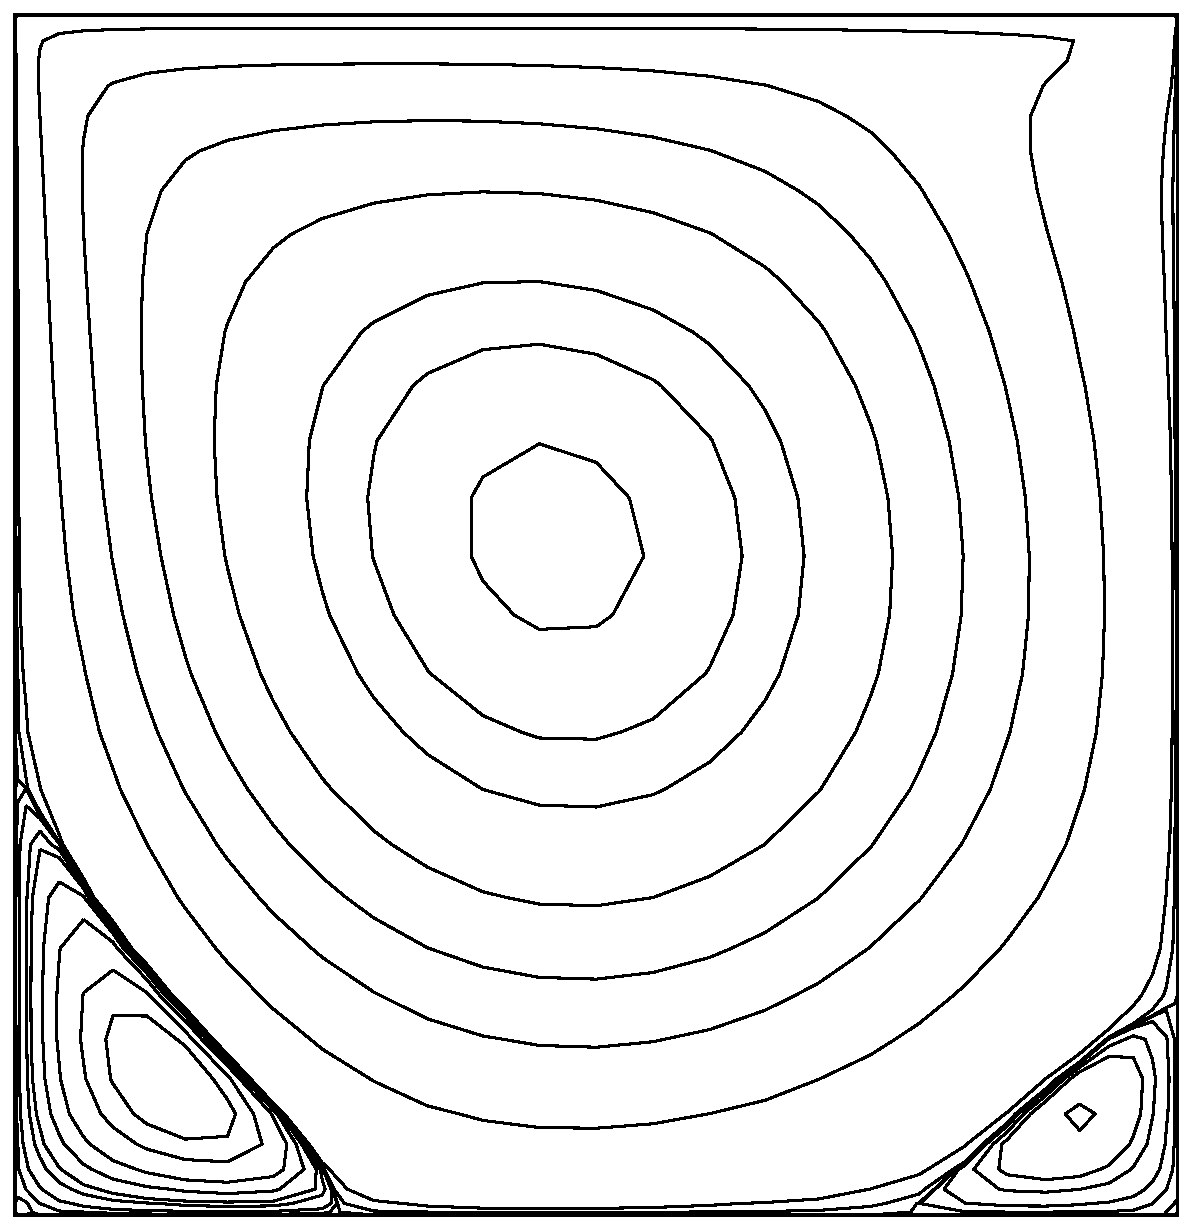
\includegraphics[width=0.95\linewidth]{Images/streamFunction32.pdf}}
	    \caption{$N = 32$}
    	\label{fig:sfe}
    \end{subfigure}
    % This comment avoids line break...
    \begin{subfigure}[b]{0.49\textwidth}
        \centering{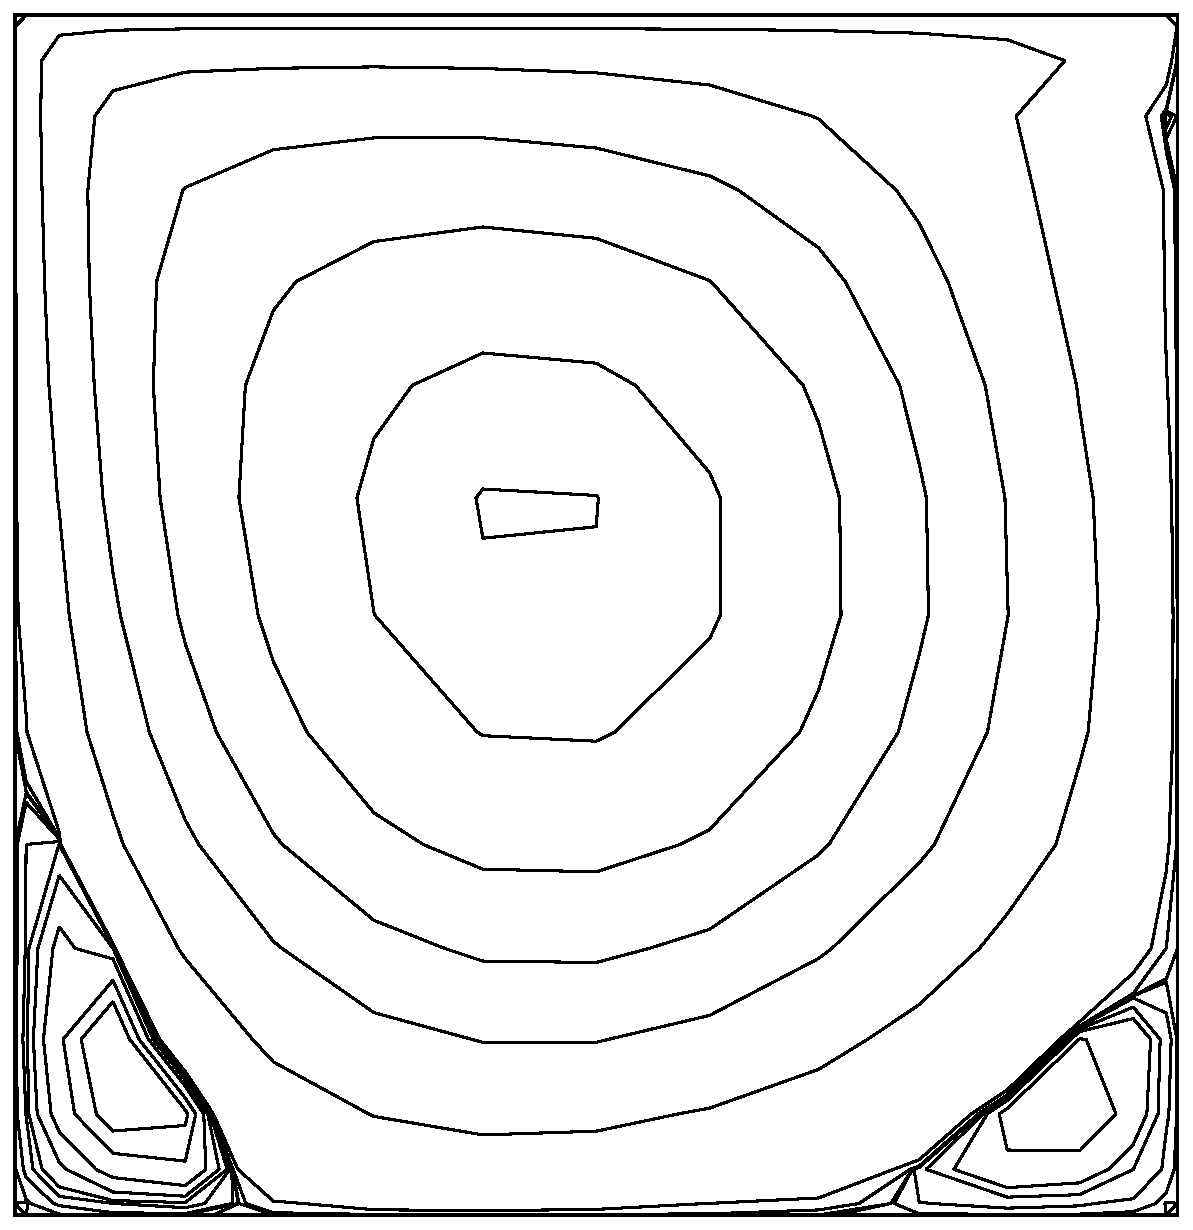
\includegraphics[width=0.95\linewidth]{Images/streamFunction16.pdf}}
	    \caption{$N = 16$}
    	\label{fig:sff}
    \end{subfigure}
    \caption{Stream function for $\text{Re} = 1000$, $\Delta t = 0.0002$, $\text{tol} = 1 \cdot 10^{-5}$, and various values of $N$ as well as the benchmark result}
    \label{fig:allsf}
\end{figure}

\begin{figure}[p]
    \centering
    \begin{subfigure}[b]{0.49\textwidth}
        \centering{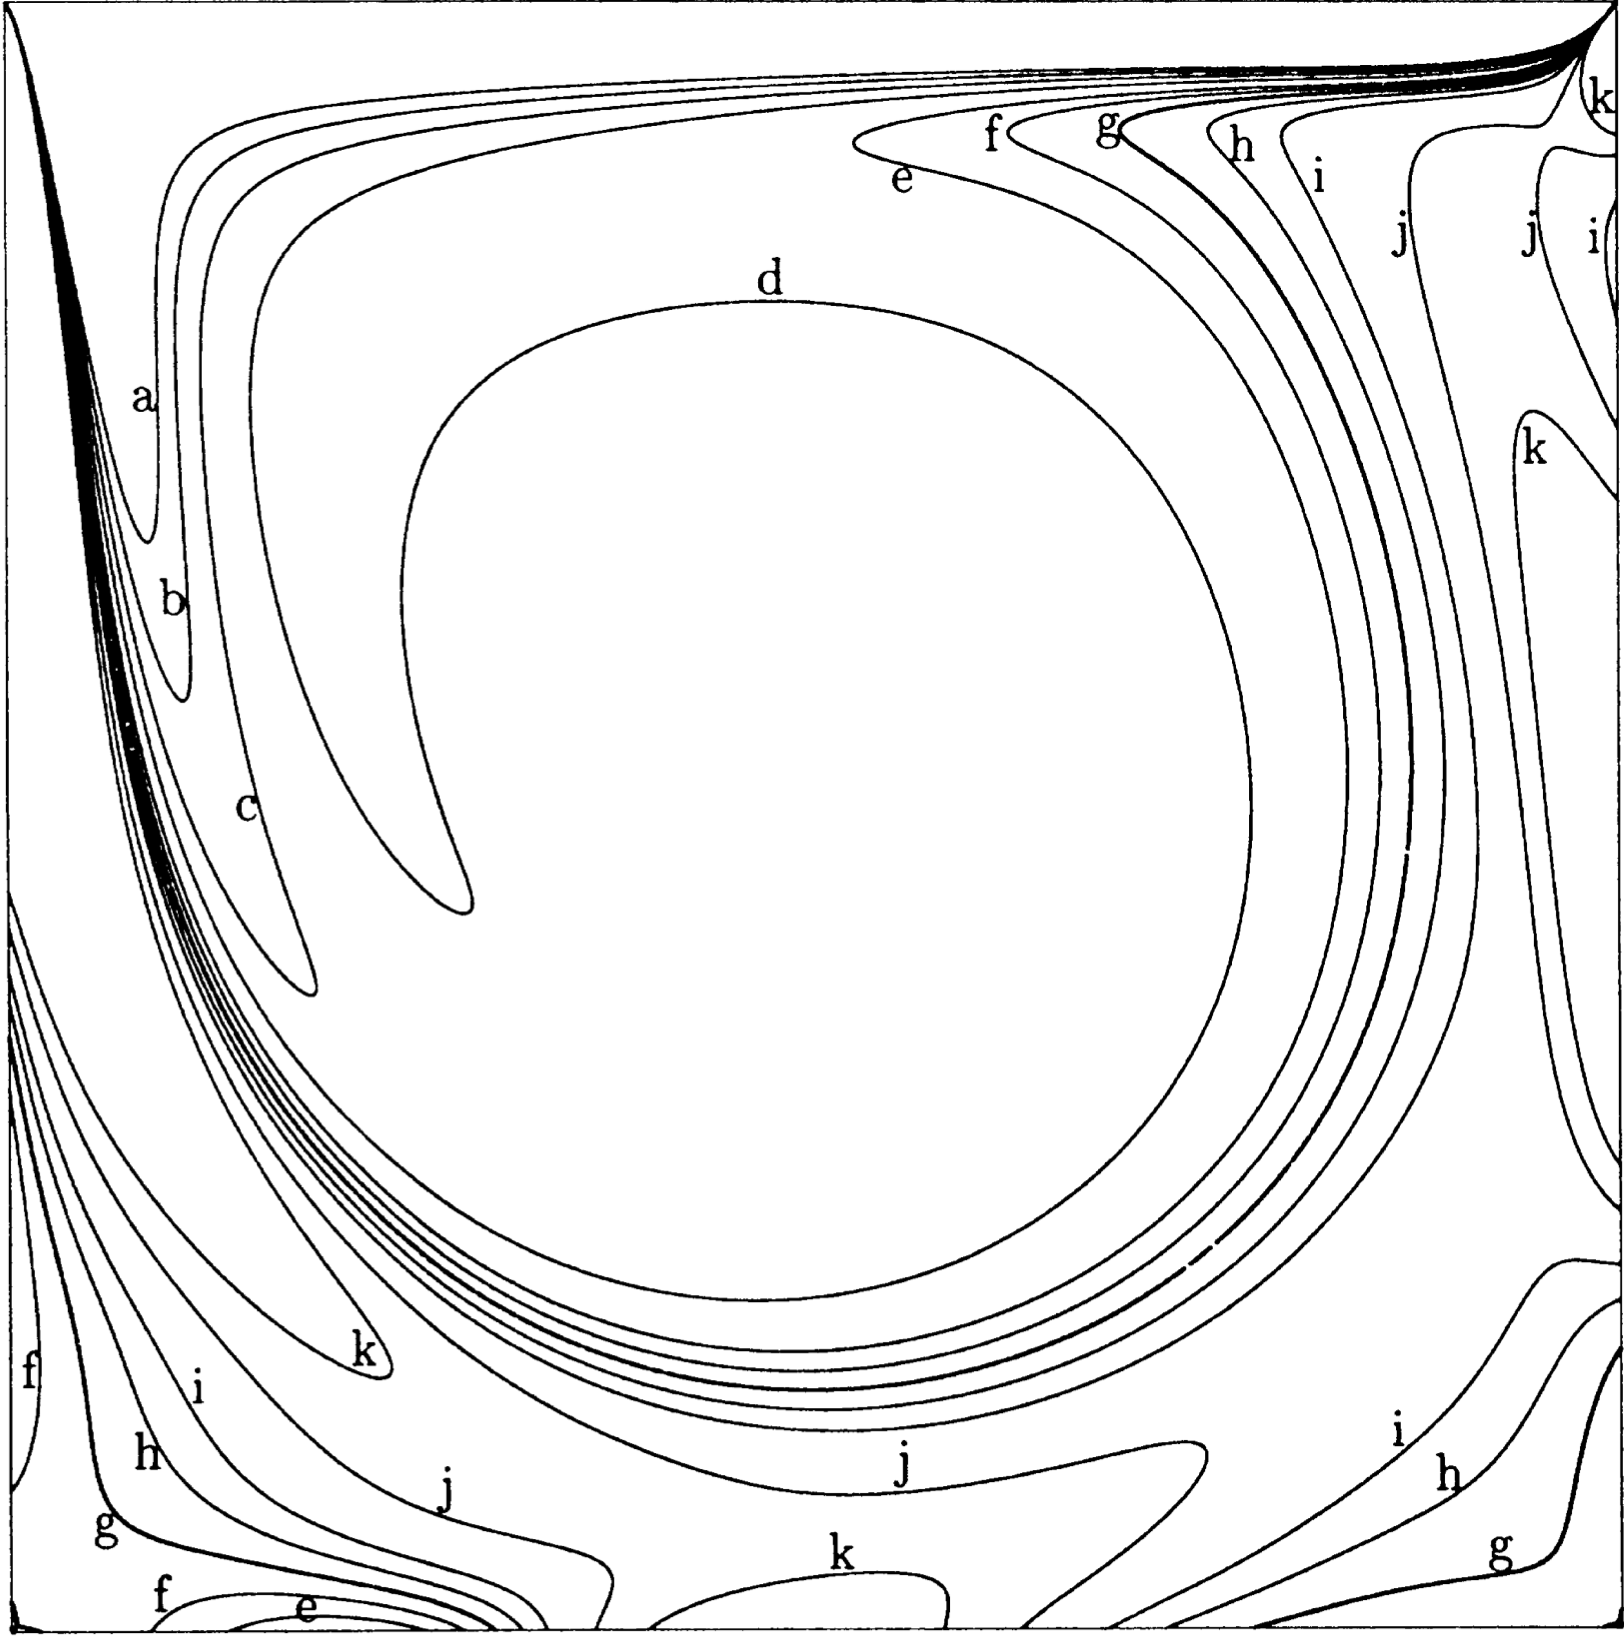
\includegraphics[width=0.95\linewidth]{Images/vorticity.png}}
	    \caption{Benchmark}
    	\label{fig:va}
    \end{subfigure}
    % This comment avoids line break...
    \begin{subfigure}[b]{0.49\textwidth}
        \centering{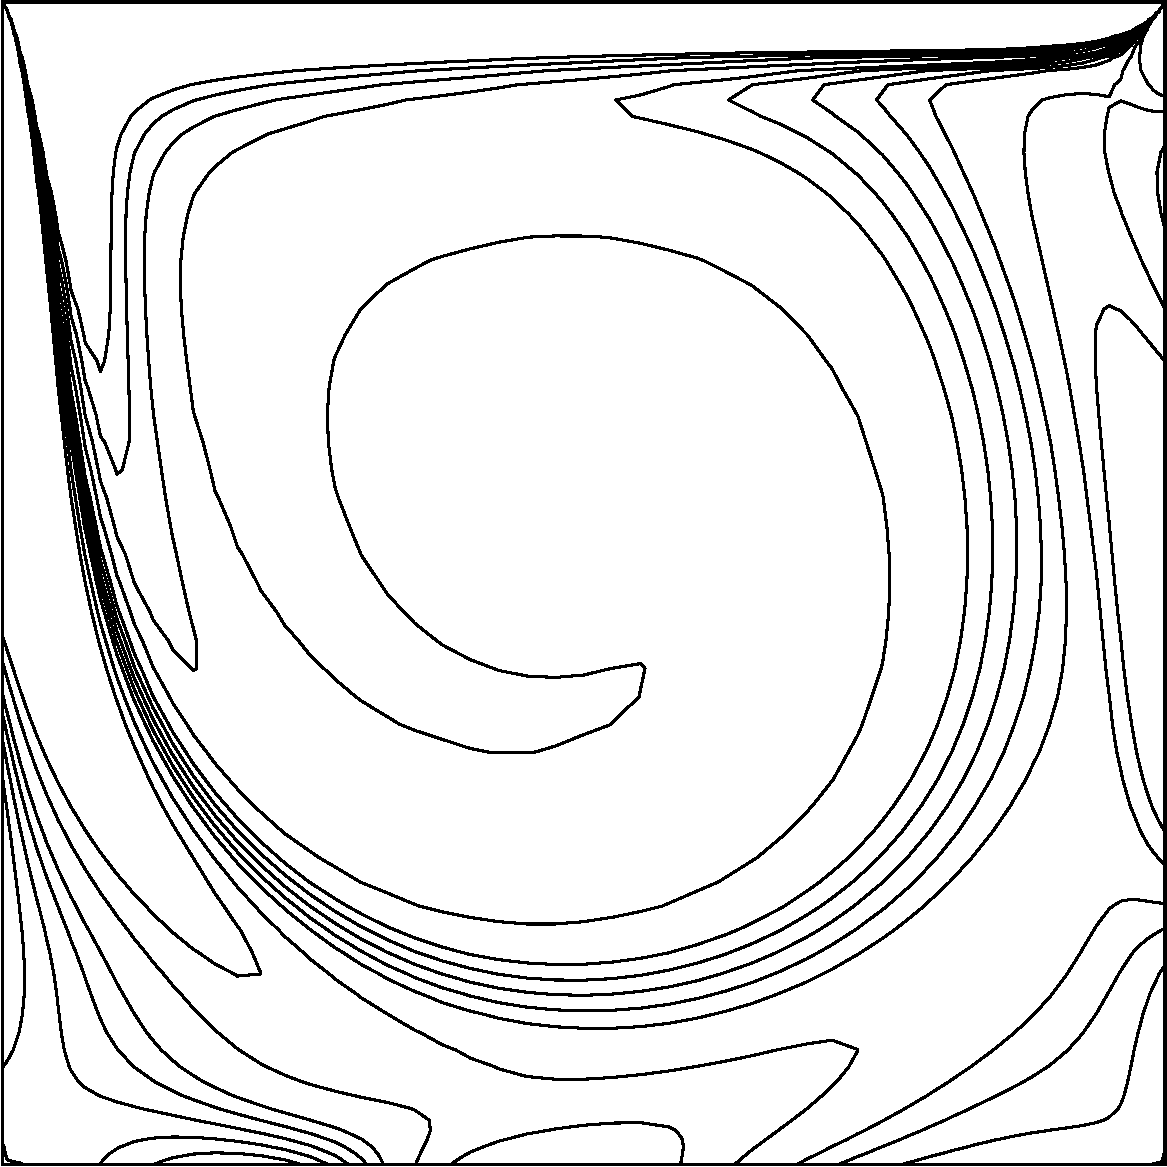
\includegraphics[width=0.95\linewidth]{Images/vorticity64.pdf}}
	    \caption{$N = 64$}
	    \label{fig:vb}	
    \end{subfigure}
    
    \vspace{1cm}
    
    \begin{subfigure}[b]{0.49\textwidth}
        \centering{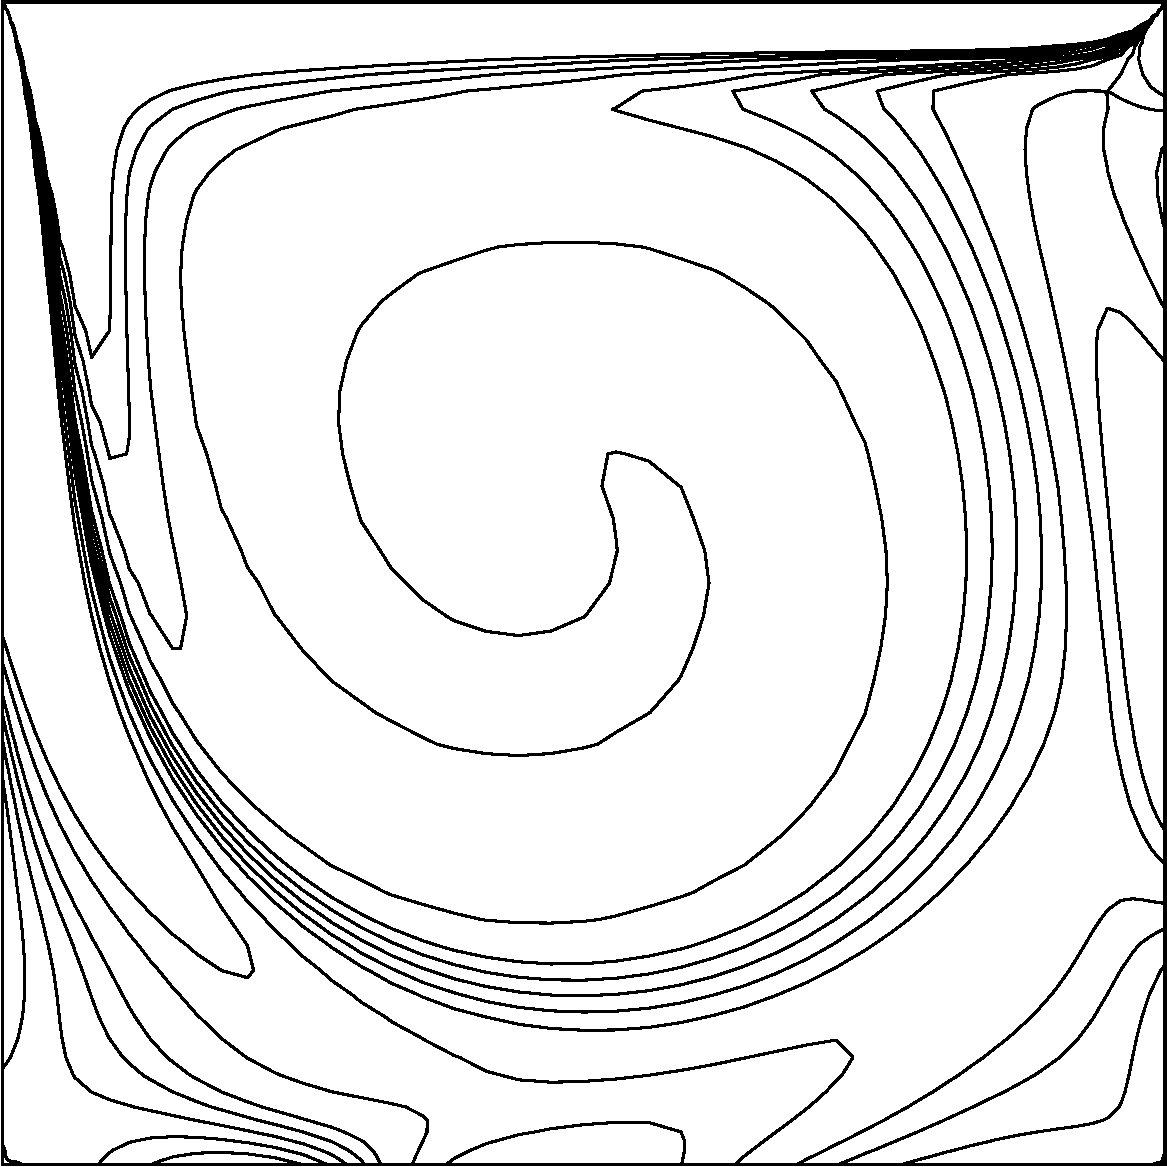
\includegraphics[width=0.95\linewidth]{Images/vorticity56.pdf}}
	    \caption{$N = 56$}
    	\label{fig:vc}
    \end{subfigure}
    % This comment avoids line break...
    \begin{subfigure}[b]{0.49\textwidth}
        \centering{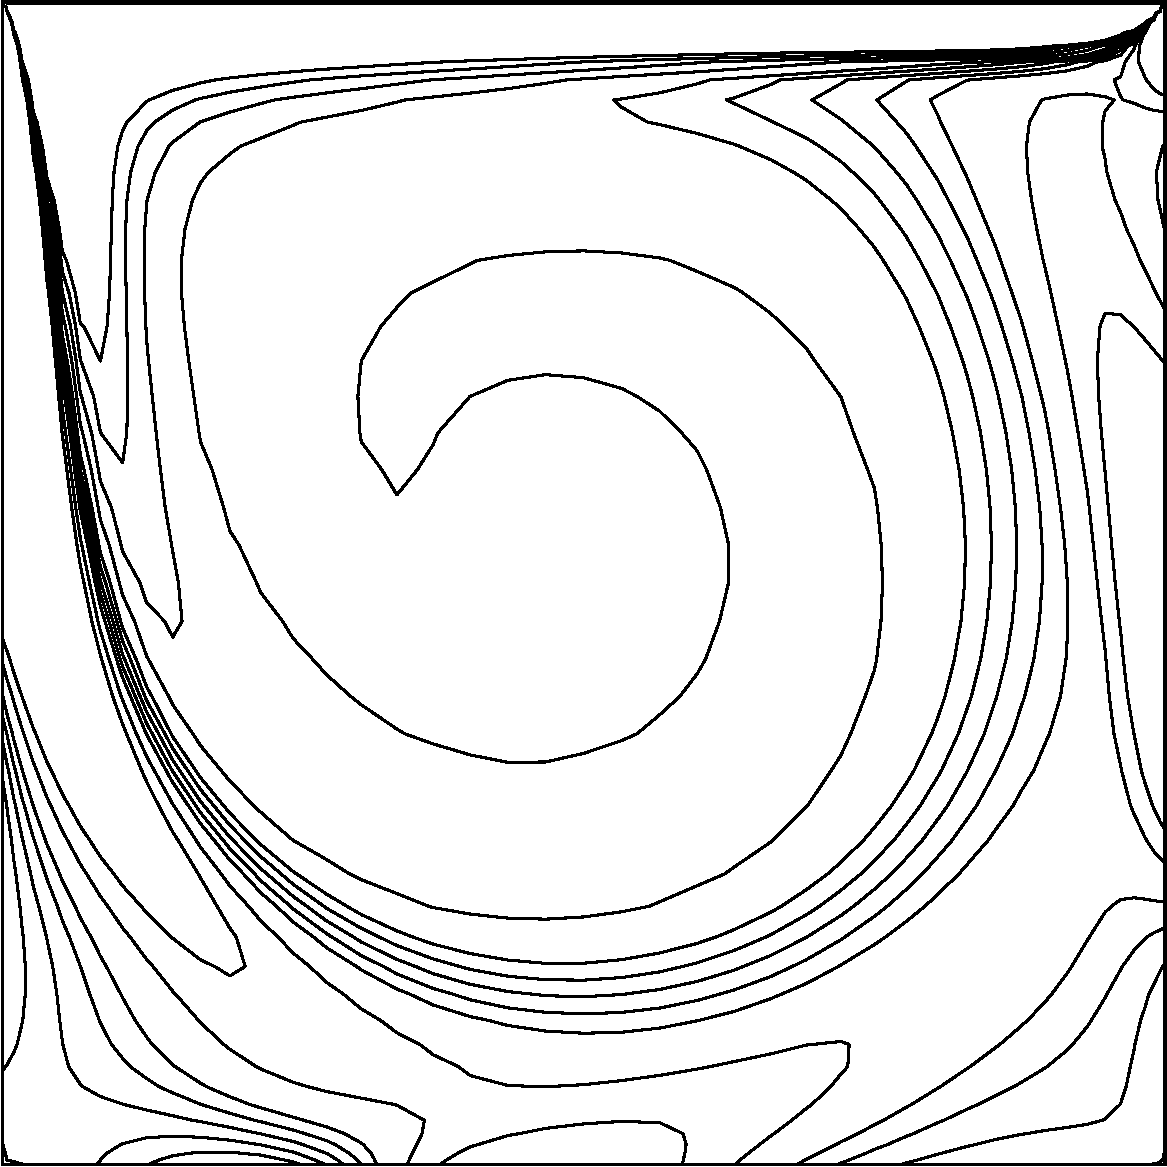
\includegraphics[width=0.95\linewidth]{Images/vorticity48.pdf}}
	    \caption{$N = 48$}
	    \label{fig:vd}	
    \end{subfigure}
    
    \vspace{1cm}
    
    \begin{subfigure}[b]{0.49\textwidth}
        \centering{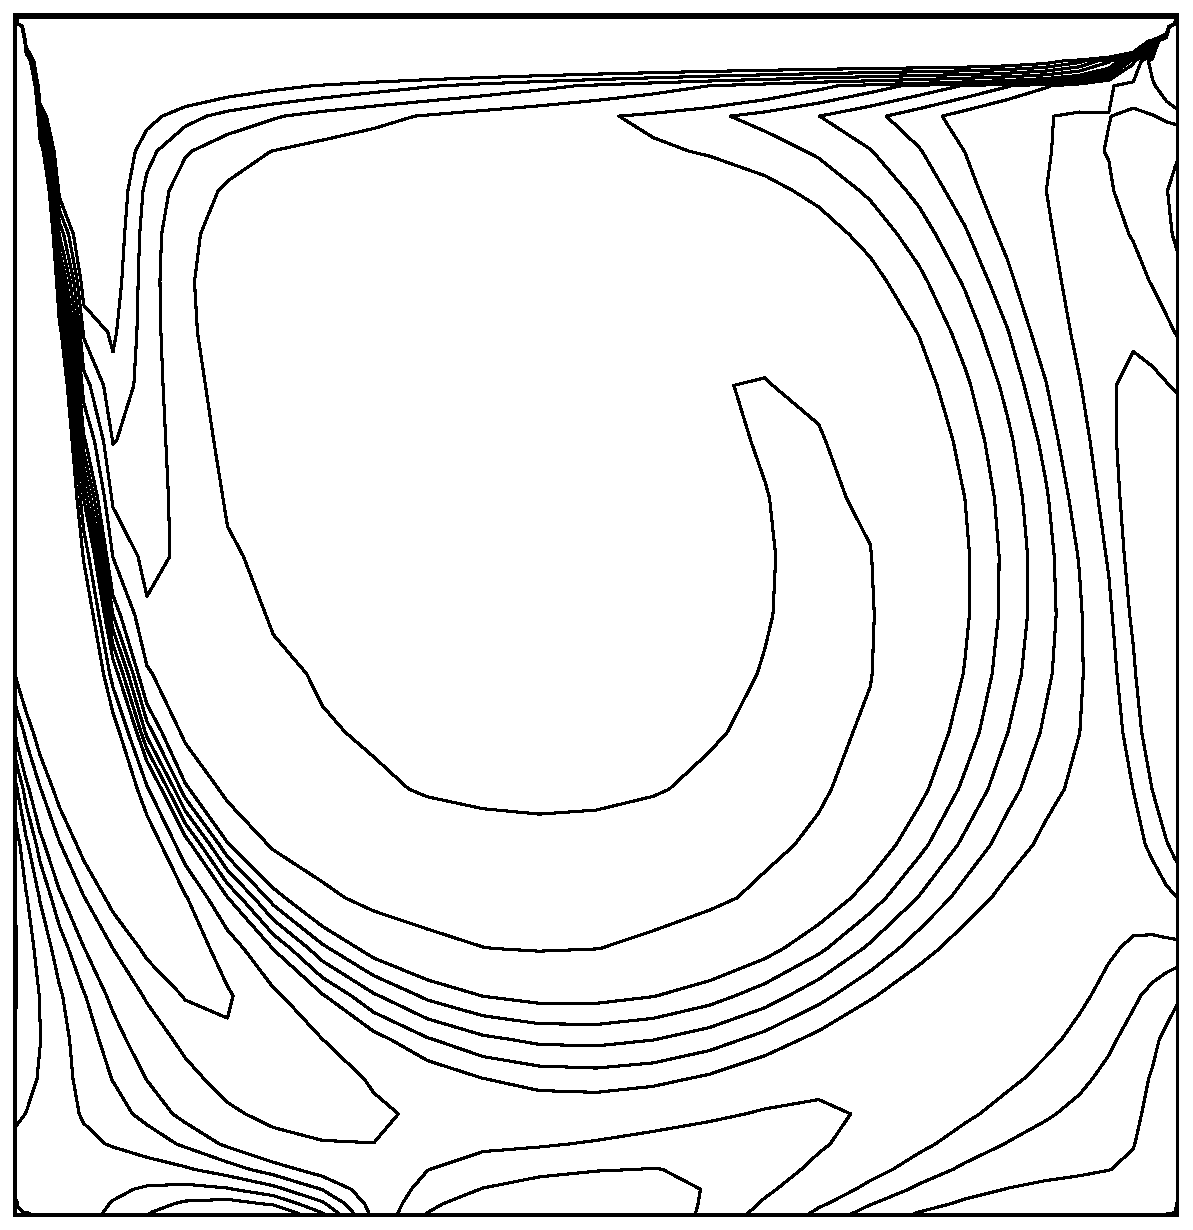
\includegraphics[width=0.95\linewidth]{Images/vorticity32.pdf}}
	    \caption{$N = 32$}
    	\label{fig:ve}
    \end{subfigure}
    % This comment avoids line break...
    \begin{subfigure}[b]{0.49\textwidth}
        \centering{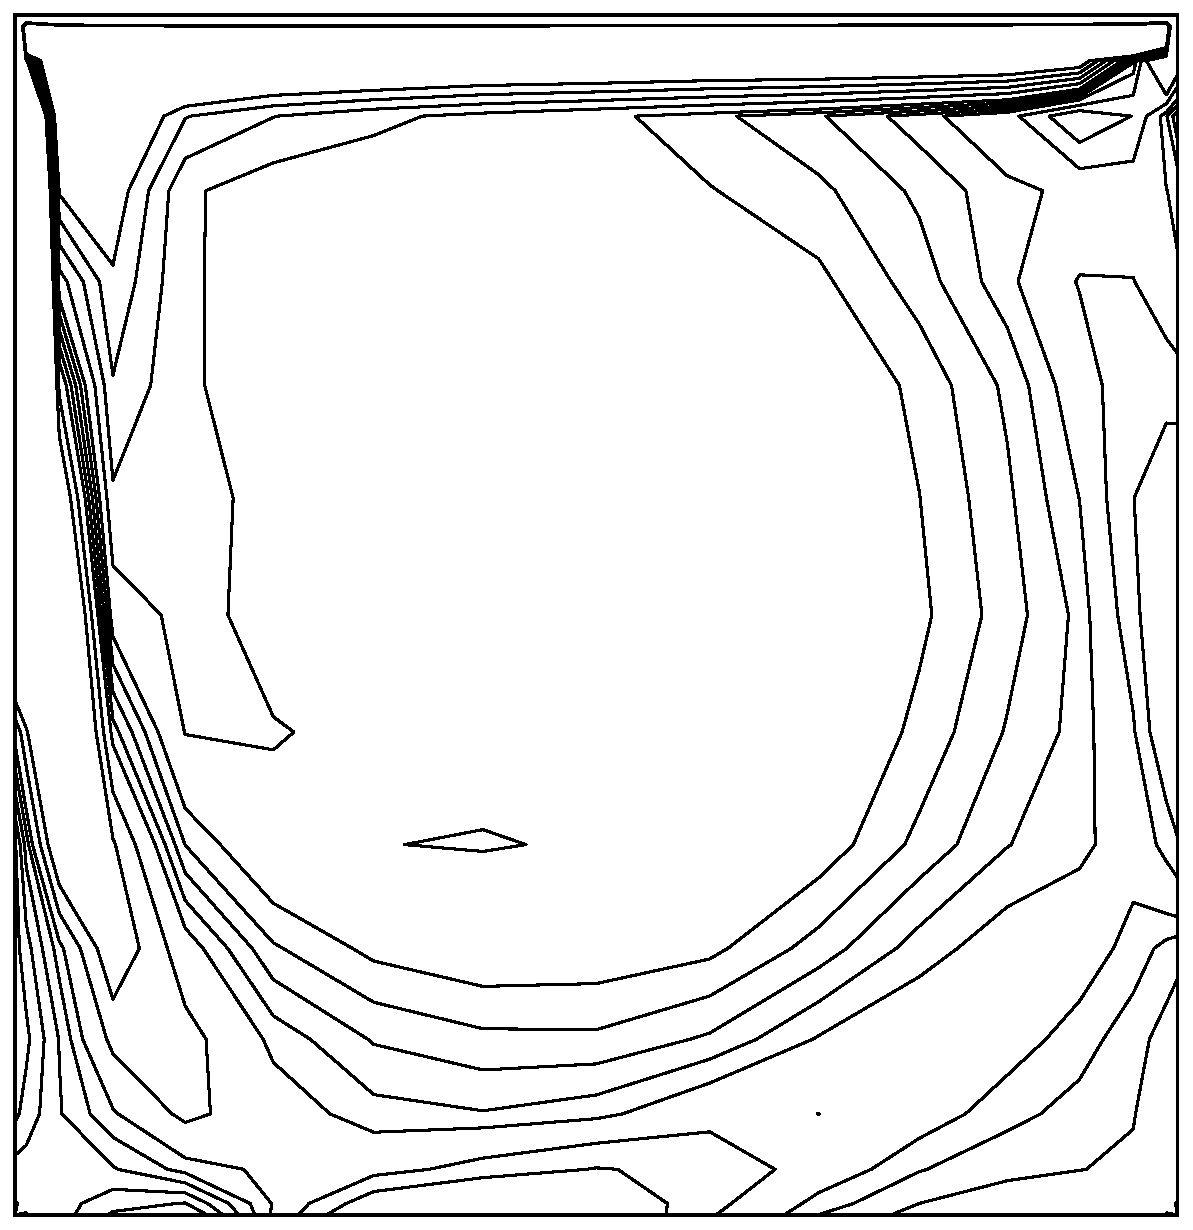
\includegraphics[width=0.95\linewidth]{Images/vorticity16.pdf}}
	    \caption{$N = 16$}
	    \label{fig:vf}
    \end{subfigure}
    \caption{Vorticity for $\text{Re} = 1000$, $\Delta t = 0.0002$, $\text{tol} = 1 \cdot 10^{-5}$, and various values of $N$ as well as the benchmark result.}
    \label{fig:allvorticity}
\end{figure}

\begin{figure}[p]
    \centering
    \begin{subfigure}[b]{0.49\textwidth}
        \centering{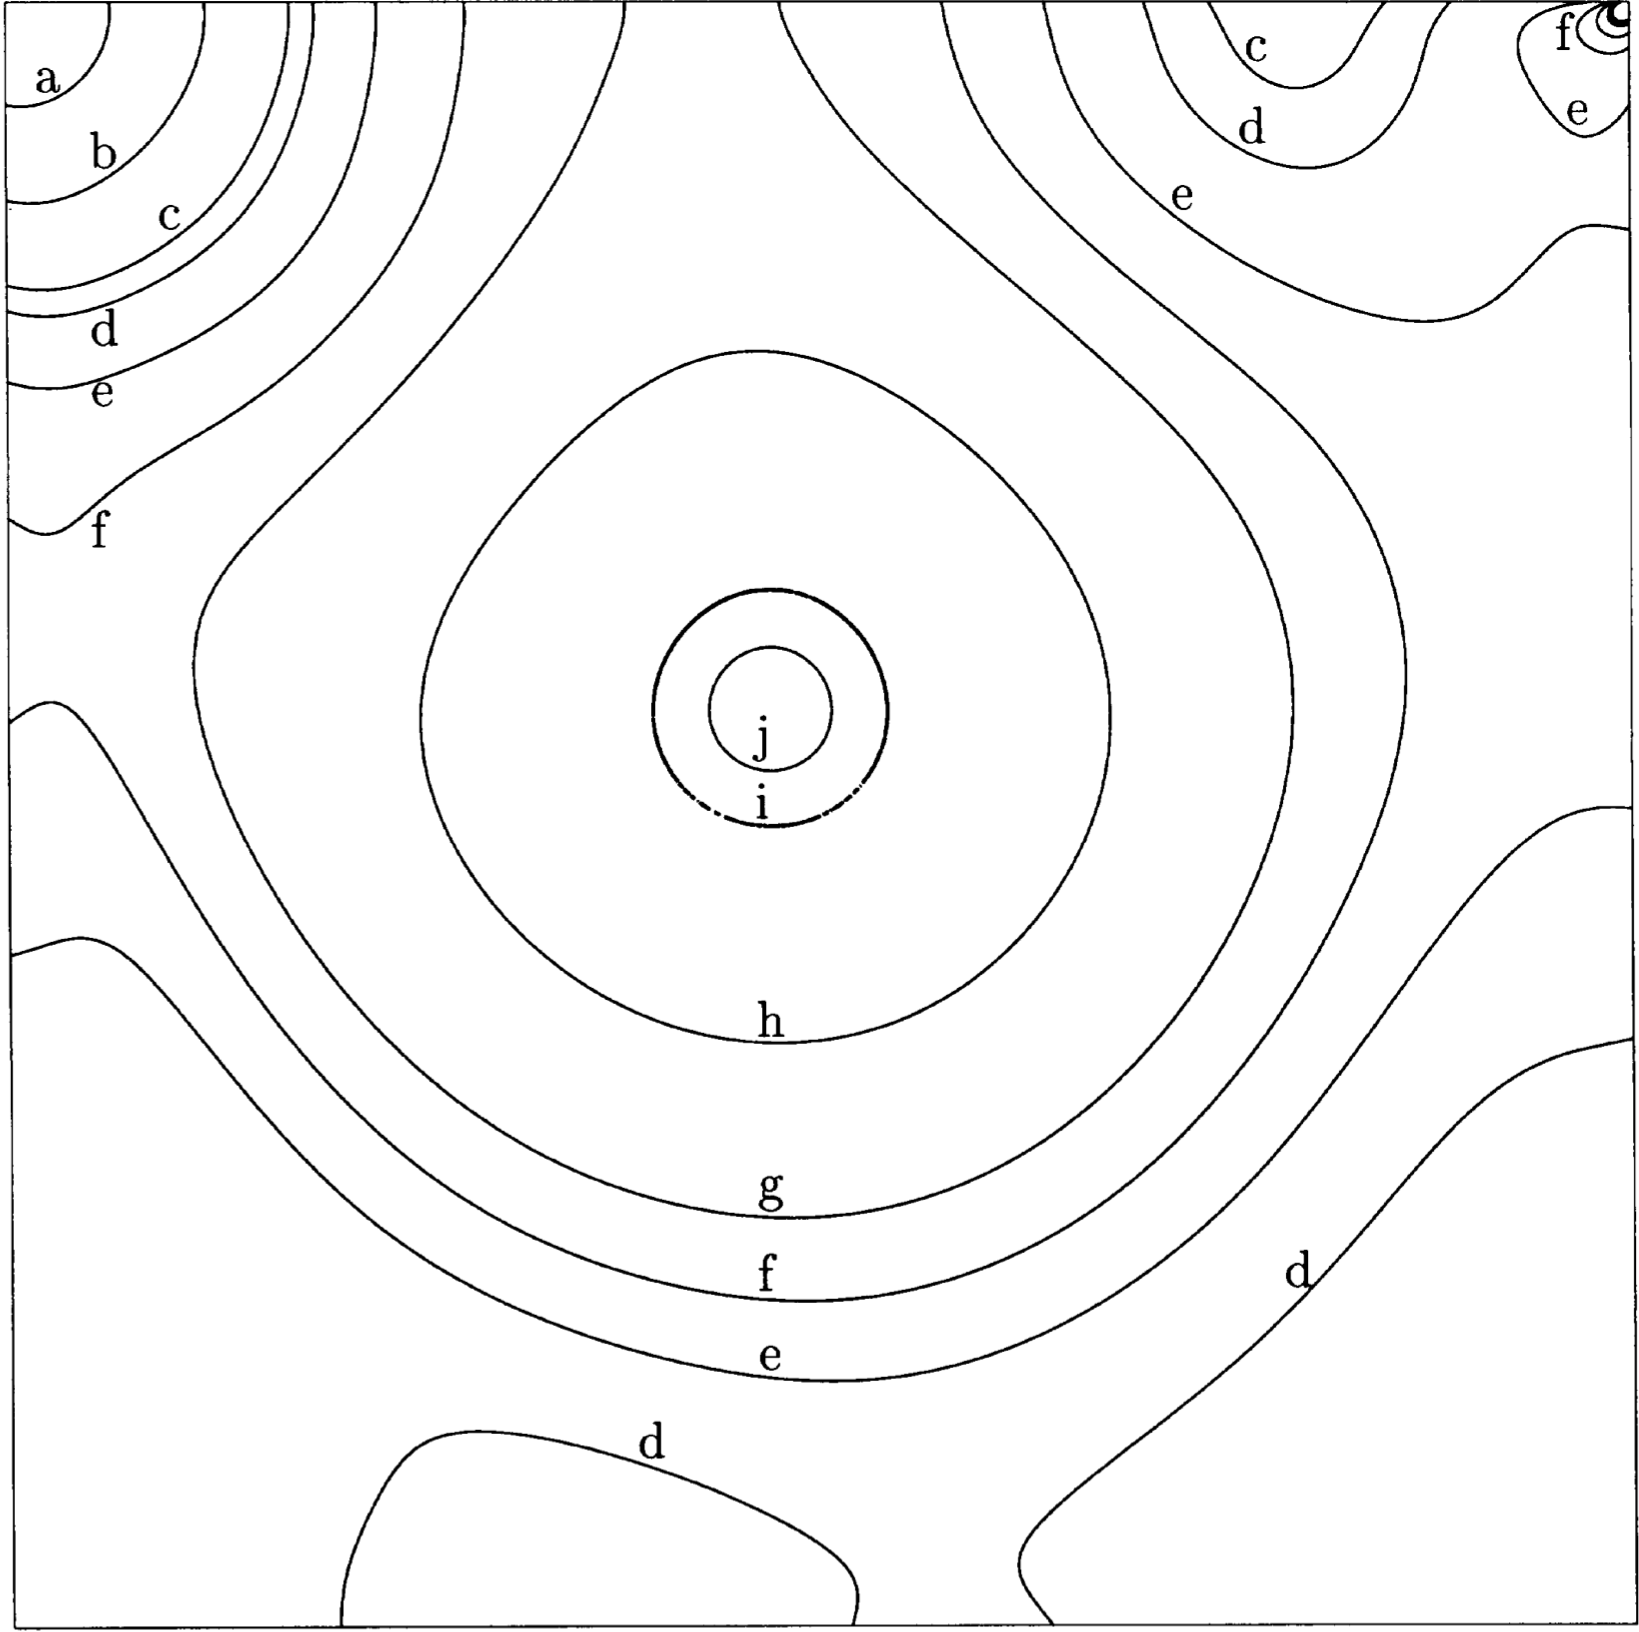
\includegraphics[width=0.95\linewidth]{Images/pressure.png}}
	    \caption{Benchmark}
    	\label{fig:pressurea}
    \end{subfigure}
    % This comment avoids line break...
    \begin{subfigure}[b]{0.49\textwidth}
        \centering{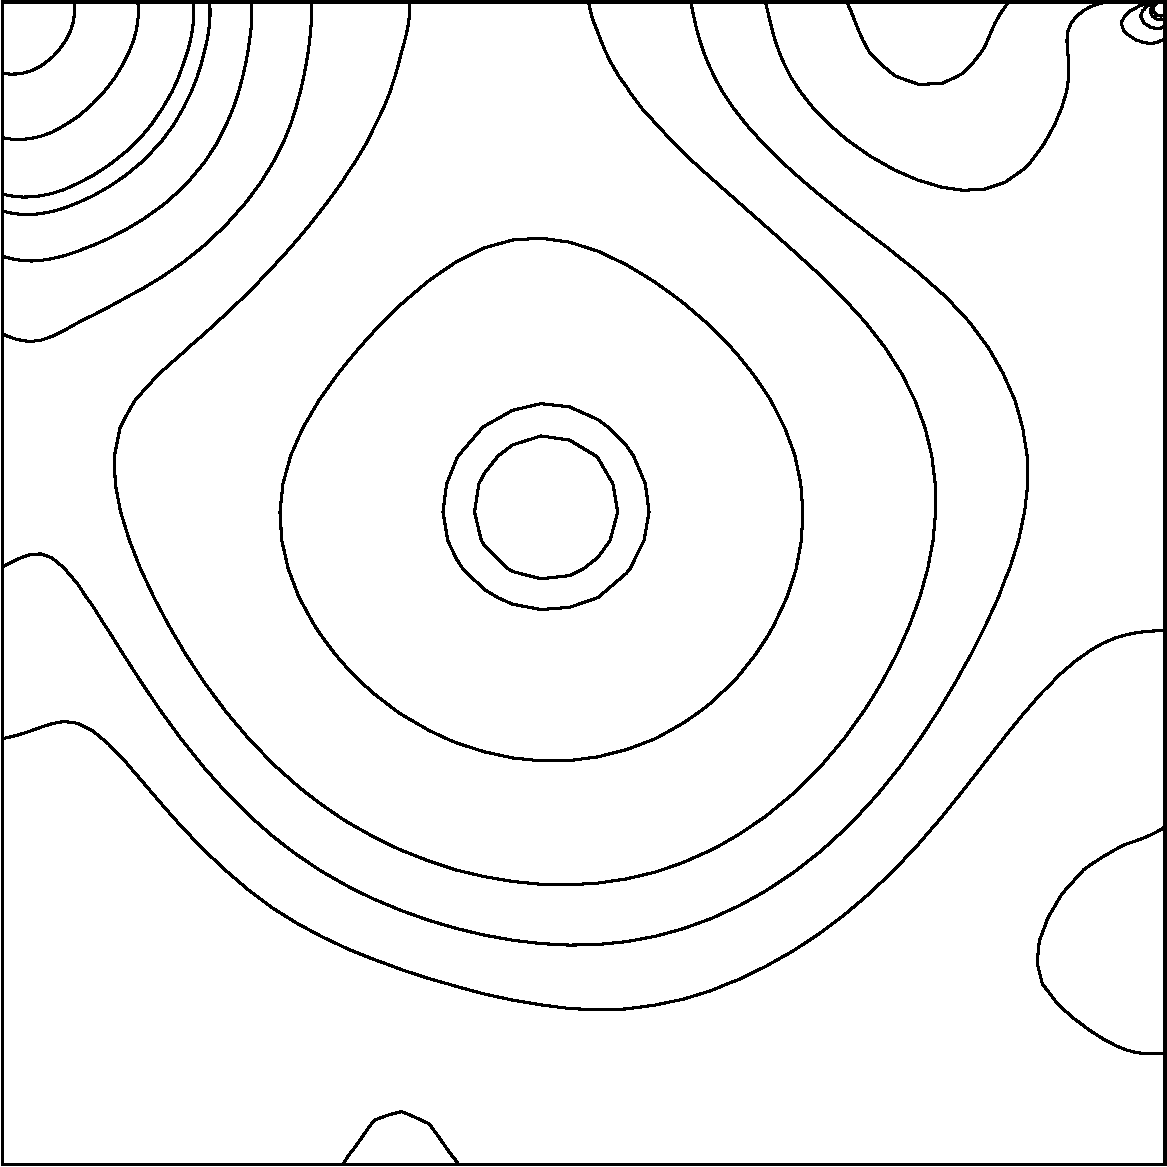
\includegraphics[width=0.95\linewidth]{Images/pressure64.pdf}}
	    \caption{$N = 64$}
	    \label{fig:pressureb}	
    \end{subfigure}
    
    \vspace{1cm}
    
    \begin{subfigure}[b]{0.49\textwidth}
        \centering{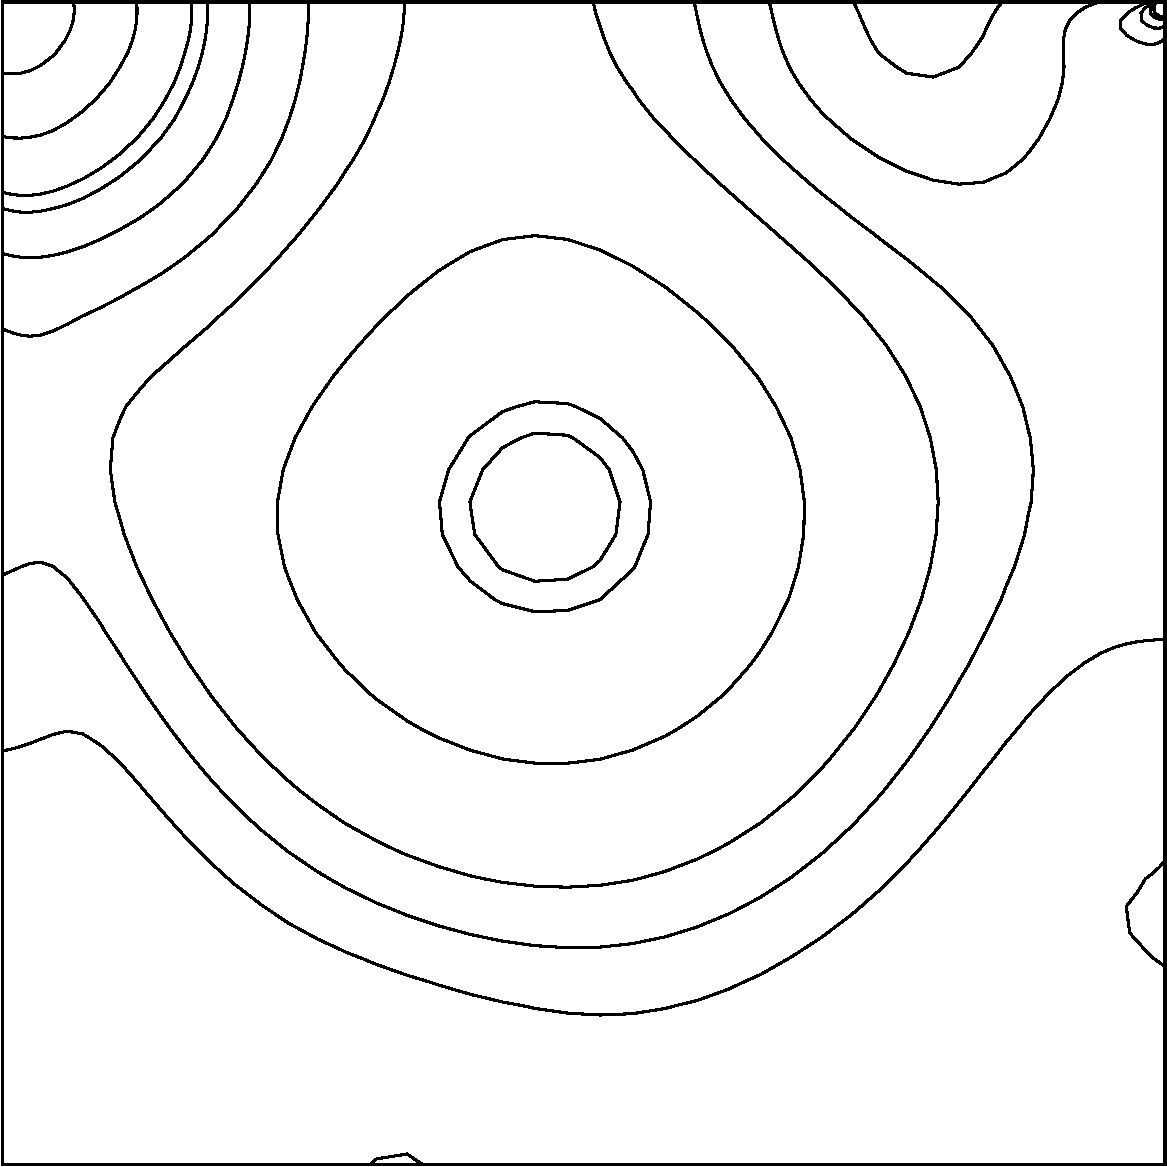
\includegraphics[width=0.95\linewidth]{Images/pressure56.pdf}}
	    \caption{$N = 56$}
    	\label{fig:pressurec}
    \end{subfigure}
    % This comment avoids line break...
    \begin{subfigure}[b]{0.49\textwidth}
        \centering{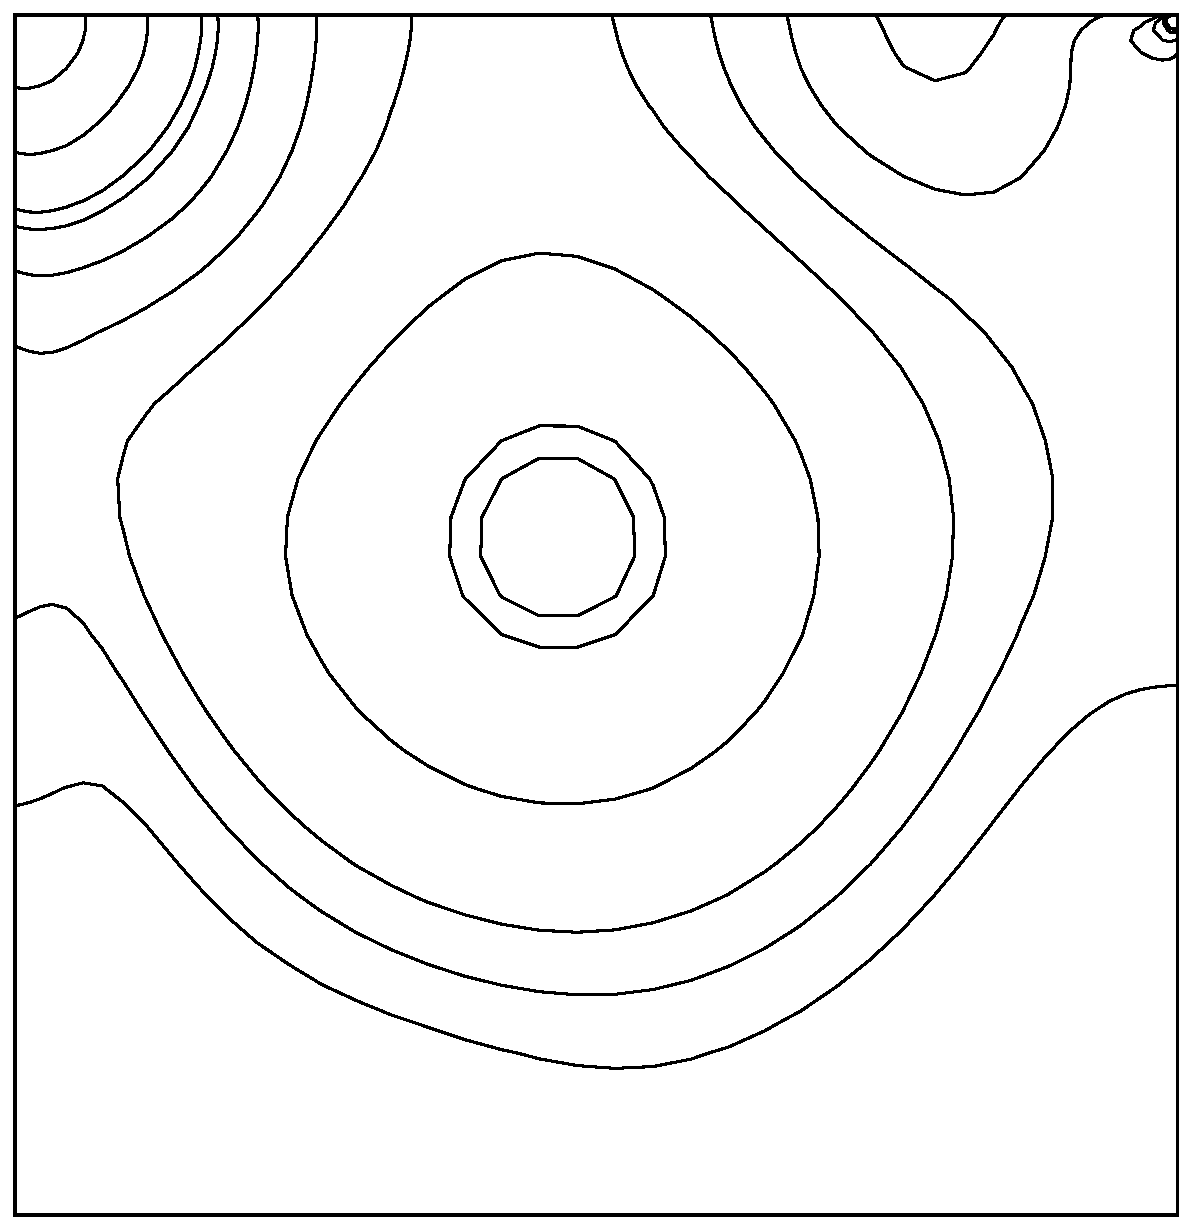
\includegraphics[width=0.95\linewidth]{Images/pressure48.pdf}}
	    \caption{$N = 48$}
	    \label{fig:pressured}	
    \end{subfigure}
    
    \vspace{1cm}
    
    \begin{subfigure}[b]{0.49\textwidth}
        \centering{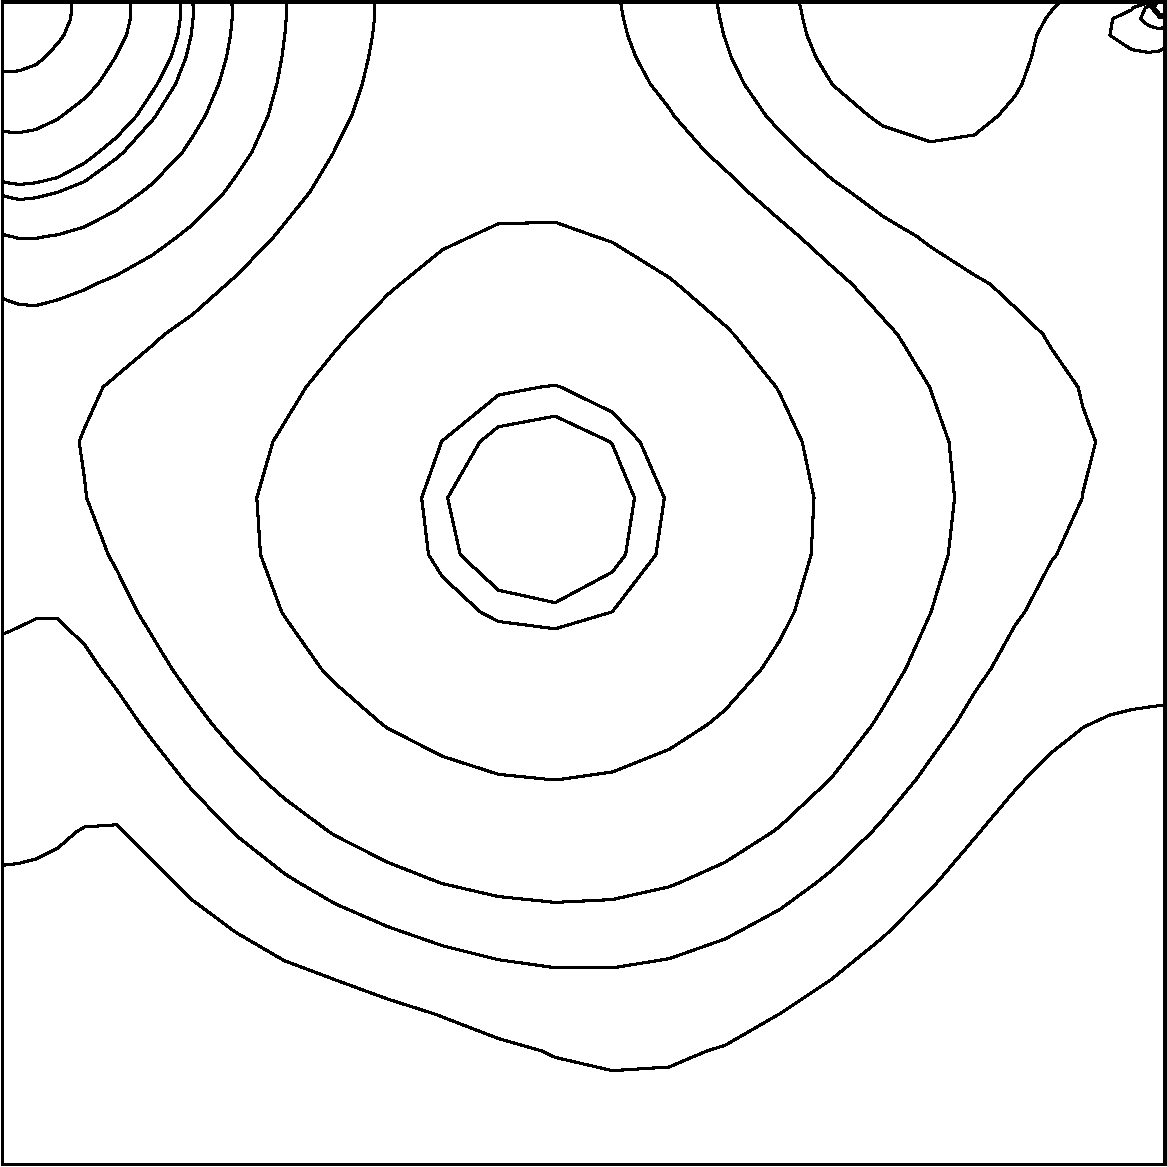
\includegraphics[width=0.95\linewidth]{Images/pressure32.pdf}}
	    \caption{$N = 32$}
    	\label{fig:pressuree}
    \end{subfigure}
    % This comment avoids line break...
    \begin{subfigure}[b]{0.49\textwidth}
        \centering{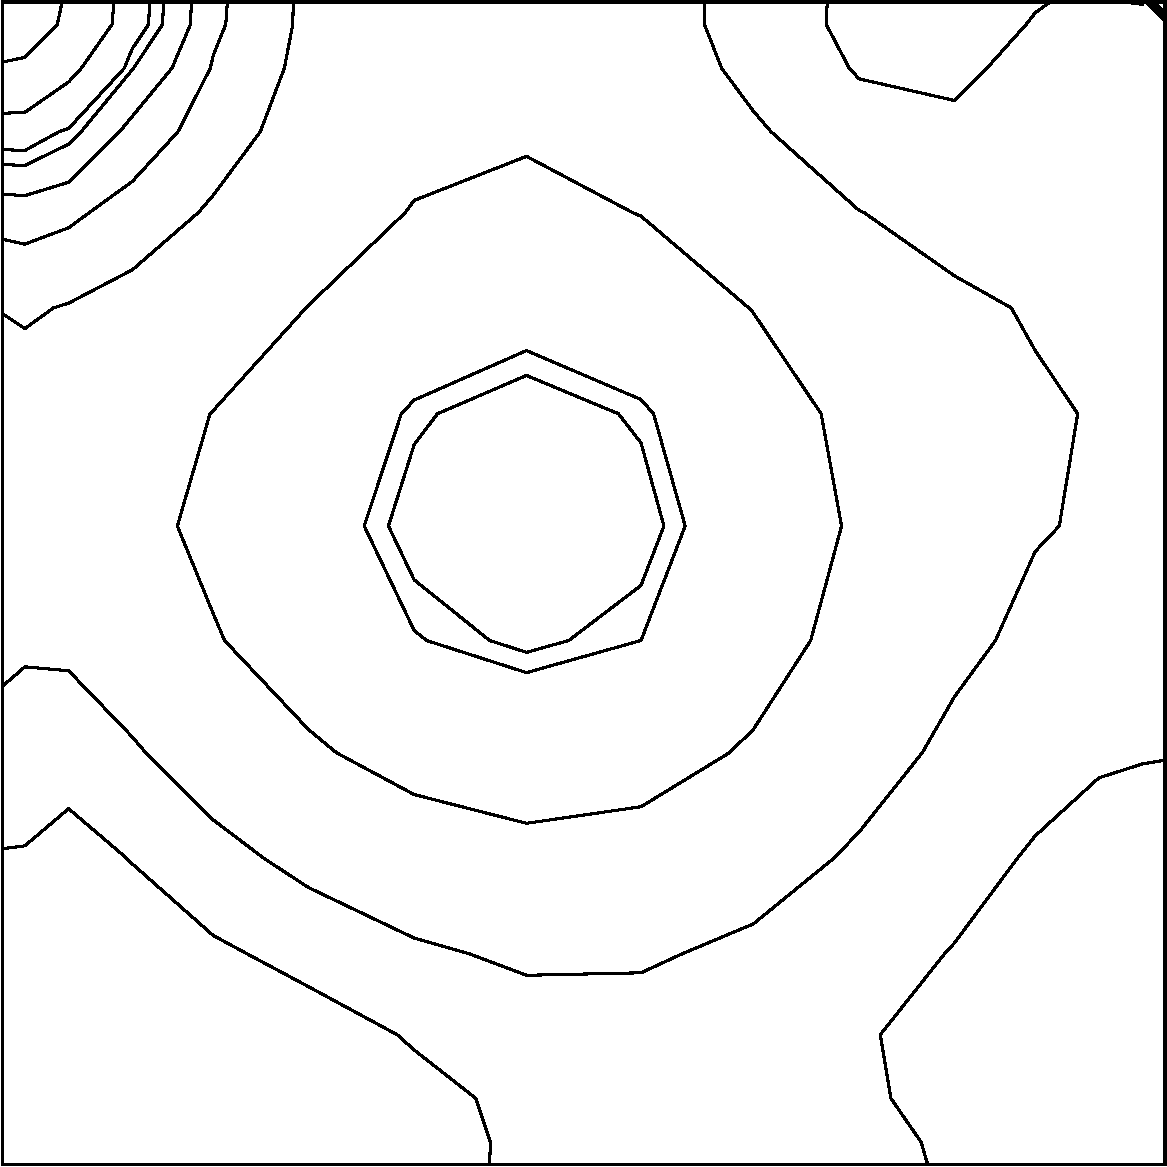
\includegraphics[width=0.95\linewidth]{Images/pressure16.pdf}}
	    \caption{$N = 16$}
	    \label{fig:pressuref}
    \end{subfigure}
    \caption{Static pressure for $\text{Re} = 1000$, $\Delta t = 0.0002$, $\text{tol} = 1 \cdot 10^{-5}$, and various values of $N$ as well as the benchmark result.}
    \label{fig:allpressure}
\end{figure}
